%%%---PREAMBLE---%%%%%%%%%%%%%%%%%%%%%%%%%%%%
\documentclass[oneside,12pt,final]{ucthesis-CA2012}
\pdfoutput=1

%--- Packages ---------------------------------------------------------
\usepackage[lofdepth,lotdepth,caption=false]{subfig}
\usepackage{fancyhdr}
\usepackage{hyperref}
\usepackage{amsmath, amssymb, graphicx}
\usepackage{xspace}
\usepackage{braket}
\usepackage{color}
\usepackage{setspace}
%\usepackage{subfigure} (Subfigure package clashes with another package)

%---New Definitions and Commands------------------------------------------------------
\def\p{\partial}
\def\im{\mrm{im}}
\def\Tr{\mrm{Tr}}
\def\Z{\mbb{Z}}
\def\R{\mbb{R}}
\def\C{\mbb{C}}
\def\half{\frac{1}{2}}
\def\filler{\phantom{fillerfillerfiller}}
\newcommand{\be}{\begin{equation}}
\newcommand{\ee}{\end{equation}}
\newcommand{\mbb}[1]{\mathbb{#1}}
\newcommand{\mrm}[1]{\mathrm{#1}}
\newcommand{\mcal}[1]{\mathcal{#1}}
\newcommand{\mbf}[1]{\mathbf{#1}}
\newcommand{\ph}[1]{\phantom{#1}}
\newcommand{\udten}[3]{#1^{#2}_{\ph{#2}#3}}
\newcommand{\duten}[3]{#1^{\ph{#2}#3}_{#2}}
\newcommand{\pd}[2]{\frac{\p#1}{\p#2}}
\newcommand{\D}[2]{\frac{d#1}{d#2}}

%---Set Margins ------------------------------------------------------
\setlength\oddsidemargin{0.25 in} \setlength\evensidemargin{0.25 in} \setlength\textwidth{6.25 in} \setlength\textheight{8.50 in}
\setlength\footskip{0.25 in} \setlength\topmargin{0 in} \setlength\headheight{0.25 in} \setlength\headsep{0.25 in}

%%%---DOCUMENT---%%%%%%%%%%%%%%%%%%%%%%%%%%%%
\begin{document}

%=== Preliminary Pages ============================================
\begin{frontmatter}
	%%%%%%%%%%%%%%%%%%%%%%%%%%%
% TITLE PAGE INFORMATION %
%%%%%%%%%%%%%%%%%%%%%%%%%%%


\title{Advancing Synthesizable Verilog/SystemVerilog Education with Open-Source Tools and Autograders}

\author{Ethan Sifferman}

%%%%%%%%%%%%%%%%%%%%%%%%%%%%%%%%%%
% DECLARATIONS FOR FRONT MATTER %
%%%%%%%%%%%%%%%%%%%%%%%%%%%%%%%%%%
\report{Thesis} \degree{Master of Computer Engineering} \degreemonth{June} \degreeyear{2023}
\defensemonth{September}
\defenseyear{2023}

\chair{Assistant Professor Jonathan Balkind}
\othermemberA{Professor Dmitri Strukov}
\othermemberB{Professor Yogananda Isukapalli}
\numberofmembers{3}

\field{Electrical and Computer Engineering}
\campus{Santa Barbara}

	\maketitle
	\approvalpage
	\copyrightpage
	\begin{vitae}
    \addcontentsline{toc}{chapter}{Curriculum Vitae}

    \begin{vitaesection}{Education}
    \vspace{-0.1cm}
    \item [Sep`23 \emph{(expected)}] M.S. in Computer Engineering, University of California, Santa Barbara
    \item [June`22] B.S. in Computer Engineering, University of California, Santa Barbara
    \end{vitaesection}

    \begin{vitaesection}{Professional Experience}
        \vspace{-0.1cm}
        \item [June`22 - Dec`22] Intel Corporation SoC Design Engineer Graduate Intern
    \end{vitaesection}

    \begin{vitaesection}{Teaching Experience}
        \vspace{-0.1cm}
        \item [Sep`22 - June`23] UCSB Electrical and Computer Engineering Department Teaching Assistant
        \item [Sep`20 - June`22] UCSB Computer Science Department Learning Assistant
    \end{vitaesection}

    \begin{vitaesection}{HDL Courses Assisted}
        \vspace{-0.1cm}
        \item [Spring`22] CS 154 -- Computer Architecture
        \item [Fall`22] ECE 154A -- Introduction to Computer Architecture
        \item [Winter`23] UCSB ECE 154B -- Advanced Computer Architecture
        \item [Spring`23] UCSB ECE 152A -- Digital Design Principles
    \end{vitaesection}

    \begin{vitaesection}{HDL Courses Instructed}
        \vspace{-0.1cm}
        \item [Spring`22] UCSB IEEE ``FPGA Screensaver Project''
    \end{vitaesection}

    \begin{vitaesection}{Miscellaneous}
        \vspace{-0.1cm}
        \item [May`23] UCSB College of Engineering Outstanding ECE TA Award, \$2,600
        \item [Mar`23] FOSSi Foundation Latch-Up Presentation, ``Using CVA6 in Architecture Education''
    \end{vitaesection}

\end{vitae}

	%
%  Abstract
%

\begin{abstract}
\addcontentsline{toc}{chapter}{Abstract}
%todo: max 350 words

Abstract text. 

%\abstractsignature
\end{abstract}



	\tableofcontents
\end{frontmatter}

\begin{mainmatter}

%---Set Headers and Footers ------------------------------------------------------
\pagestyle{fancy}
\renewcommand{\chaptermark}[1]{\markboth{{\sf #1 \hspace*{\fill} Chapter~\thechapter}}{} }
\renewcommand{\sectionmark}[1]{\markright{ {\sf Section~\thesection \hspace*{\fill} #1 }}}
\fancyhf{}

\makeatletter \if@twoside \fancyhead[LO]{\small \rightmark} \fancyhead[RE]{\small\leftmark} \else \fancyhead[LO]{\small\leftmark}
\fancyhead[RE]{\small\rightmark} \fi

\def\cleardoublepage{\clearpage\if@openright \ifodd\c@page\else
  \hbox{}
  \vspace*{\fill}
  \begin{center}
    This page intentionally left blank
  \end{center}
  \vspace{\fill}
  \thispagestyle{plain}
  \newpage
  \fi \fi}
\makeatother
\fancyfoot[c]{\textrm{\textup{\thepage}}} % page number
\fancyfoot[C]{\thepage}
\renewcommand{\headrulewidth}{0.4pt}

\fancypagestyle{plain} { \fancyhf{} \fancyfoot[C]{\thepage}
\renewcommand{\headrulewidth}{0pt}
\renewcommand{\footrulewidth}{0pt}}

%=== Chapters ============================================

\chapter{Introduction}

Words

Words2

\begin{section}{Permissions and Attributions}
\begin{enumerate}

\item The content of chapter 2 and appendix A is the result of a collaboration with Alice and Bob, and has previously appeared in the (Journal) (paper citation). It is reproduced here with the permission of (Institution): \url{http://}.

\end{enumerate}
\end{section}


\chapter{Advantages of Open-Source Tools in Education}
\label{chapter:open_source_tools}

Although proprietary Verilog tools are predominant in industry and often boast a wide assortment of features, I argue that they can be one of the biggest deterrents for those first learning digital design. Whether students become aghast at the preposterous licensing fees or become hung up on the steep learning curve of the interfaces, the most popular Verilog tools often have trouble exciting students into furthering their Verilog education. Fortunately, there are several open-source Verilog tools that are praised for their accessibility and ease-of-use. A valuable resource for open-source hardware tools, generators, and reusable designs can be found in the curated list provided here: \url{https://github.com/aolofsson/awesome-opensource-hardware} \cite{awesomeOpenSourceHardware}. For example, a common collection of tools include the simulators Icarus \cite{icarusGitHub} and Verilator \cite{verilatorGitHub}, the waveform viewer GTKWave \cite{gtkwaveGitHub}, the synthesis tool Yosys \cite{yosysGitHub}, the FPGA place and route tools Nextpnr \cite{nextpnrGitHub} and VTR \cite{vtrGitHub}, the ASIC flow OpenLane \cite{OpenLaneGitHub}, and the hardware package manager and build system FuseSoC \cite{fusesocGitHub, edalizeGitHub}. In this chapter, I explain why open-source tools excel over proprietary tools in introducing Verilog and digital design to students.

\section{Proprietary tool prices deter students.}

Many students choose to pursue a degree in computer engineering due to the plethora of creative outlets that it introduces them to. Consider the hands-on process of purchasing affordable circuit components for breadboards. Likewise, platforms like Arduinos and Raspberry Pis are often explored alongside the utilization of programming languages such as C++, Python, and JavaScript. The accessibility and low cost of these mediums often foster self-directed learning. Similarly, introductory Verilog courses can serve as yet another avenue for creative expression, particularly when orchestrated using free and open-source tools. However, a significant obstruction emerges when proprietary alternatives such as Questa, VCS, and Xcelium, coupled with licensing fees over \$5,000 \cite{olofssonLatchUp, licensePricesReddit}, become the focal point of a student's introduction to Verilog. Such financial barriers can easily deter enthusiasm for self-guided learning, particularly when students anticipate losing access to the software upon graduation. This is likely the reason why several students in UC Santa Barbara's Verilog courses choose to disobey the requirement of using ModelSim, and instead use Icarus and GTKWave. Students do not want to feel like their time is wasted learning a tool if they lose access to it upon graduation.

\section{Open-source tools are easy to install.}

Even if students do not want to expand their arsenal of tools for expressing their creativity, it is still important to keep Verilog tools accessible by improving students' first-time user experience. For example, Vivado is infamous for its tedious and complex installation process while taking up over 16-60GB when installed. This is contrasted with the overall positive first-time user experience that open-source tools offer. For example, with the \enquote{OSS CAD Suite} project \cite{osscadsuitebuildGitHub}, you can download all the latest binaries of the most popular open-source Verilog tools in under a minute. This beats Vivado's complicated installation process by a mile and is more-likely to remain on student's computers after the course is over since all the tools only take up half a gigabyte, as opposed to the 16-60GB that Vivado requires.

\section{Unique benefits and features of open-source tools.}

Undoubtedly, proprietary tools offer a multitude of functionalities for advanced users that open-source tools cannot offer. However, open-source tools offer many unique features that are often better for beginners. For example, Icarus runs short simulations much faster than proprietary simulators, making it perfect for receiving instant feedback as students are still learning the language syntax. Similarly, Yosys and Nextpnr perform synthesis and layout significantly faster than tools such as Vivado and Design Compiler, allowing for more rapid prototyping. Also, while ModelSim may happily parse and simulate unsynthesizable code, Verilator will give much more strict warnings, helping to demonstrate the syntax and features that should be allowed in synthesizable designs. (This is further discussed in \autoref{section:style_guides}).

But possibly the most important attribute of open-source tools is that they get updates every day, and offer full transparency when reporting bugs and requesting new features. Depending on the difficulty of the request, the tool maintainers may complete the request within a few weeks. Instructors may even decide they want to do a pull-request themselves; I personally have made several contributions to multiple tools (see \autoref{appx:contributions}). This is contrasted with the fact that many universities are not always running the most up-to-date proprietary software. For example, as of 9/10/23, UC Santa Barbara's Engineering Computing Infrastructure's latest version of ModelSim is 10.7d from April 2019, which does not support width-casting from parameters. This negatively affected one of the UCSB Spring 2023 ECE 152A labs. Bugs in tools will undoubtedly happen, but the only solution Siemens offers is to pay for an updated version with the bug fixed. Contrast this with submitting a GitHub issue with Verilator, and having the bug fixed by the next time the course is offered. Open-source tools are often simply the better choice for instructors and students alike.

\section{Avoid graphical user interfaces.}

One of the most important ways to make Verilog more accessible is by guiding students to use command line interfaces (CLIs). Nearly all large-scale Verilog designs are paired with user-friendly build scripts and Makefiles for running simulation and synthesis. This is contrasted with complex graphical user interfaces in tools like Vivado, ModelSim, VCS, and Quartus, which can feel daunting for beginners due to the number of options that users have direct access to. UC Santa Cruz Professor Dustin Richmond compares learning Vivado to being stuck in a \enquote{point-and-click adventure game} in his talk \enquote{So, you want to be an open sourcerer?} \cite{RichmondLatchUp}. By using CLIs, you can abstract away and decouple tool-specifics from digital design concepts.

To aid in the usually lengthy crafting of TCL scripts and Makefiles, an extremely powerful pair of open-source tools named FuseSoC and Edalize \cite{fusesocGitHub, edalizeGitHub} attempt to standardize build files for all Verilog tools with a central \mintinline{bash}{.core} file. The \mintinline{bash}{.core} file, interpretable by FuseSoC, contains the \enquote{run} specifications, which are then seamlessly communicated to Edalize for automated generation and execution of build scripts. FuseSoC is compatible with nearly every Verilog tool, so switching simulators is often as easy as changing one line of code in the \mintinline{bash}{.core} file. While TAing for UCSB's ECE 152A, 154A, and 154B, I capitalized on the utility of FuseSoC and Edalize to substantially accelerate assignment setup time. I could provide students with the Makefile automatically generated by Edalize, or I could provide the \mintinline{bash}{.core} file for students to run themselves with FuseSoC. Either option was effective in simplifying the build process so students could better focus on the learning-goals of the assignments.


\chapter{Using SystemVerilog for Digital Design Education}
\label{chapter:digital_design}

Navigating the realm of Verilog/SystemVerilog education presents a distinctive challenge: effectively bridging the gap between abstract Verilog syntax and tangible hardware implementations.
Teaching this intuition is of paramount importance, as it can equip aspiring electrical engineers with a deep comprehension of digital circuits, while giving them the hard-skills in computer-aided circuit creation.
While it may feel there is a trade-off between teaching Verilog design strategies and teaching circuit design strategies, I argue that teaching inference and synthesis of Verilog will actually augment student understanding of more advanced digital circuit concepts.
I would compare this to a programming course using C++ to teach algorithms.
For many computer science students, algorithms are synonymous with code, not with logic proofs.
For computer engineering students, \ul{as long as Verilog is taught with a synthesis-oriented approach, the connection between theoretical circuit concepts and tangible hardware construction becomes seamless, facilitating a more rapid and all-encompassing digital design education.}

\section{Netlist graph viewers teach Verilog inference intuition.}


\begin{figure}[t]
    \centering
    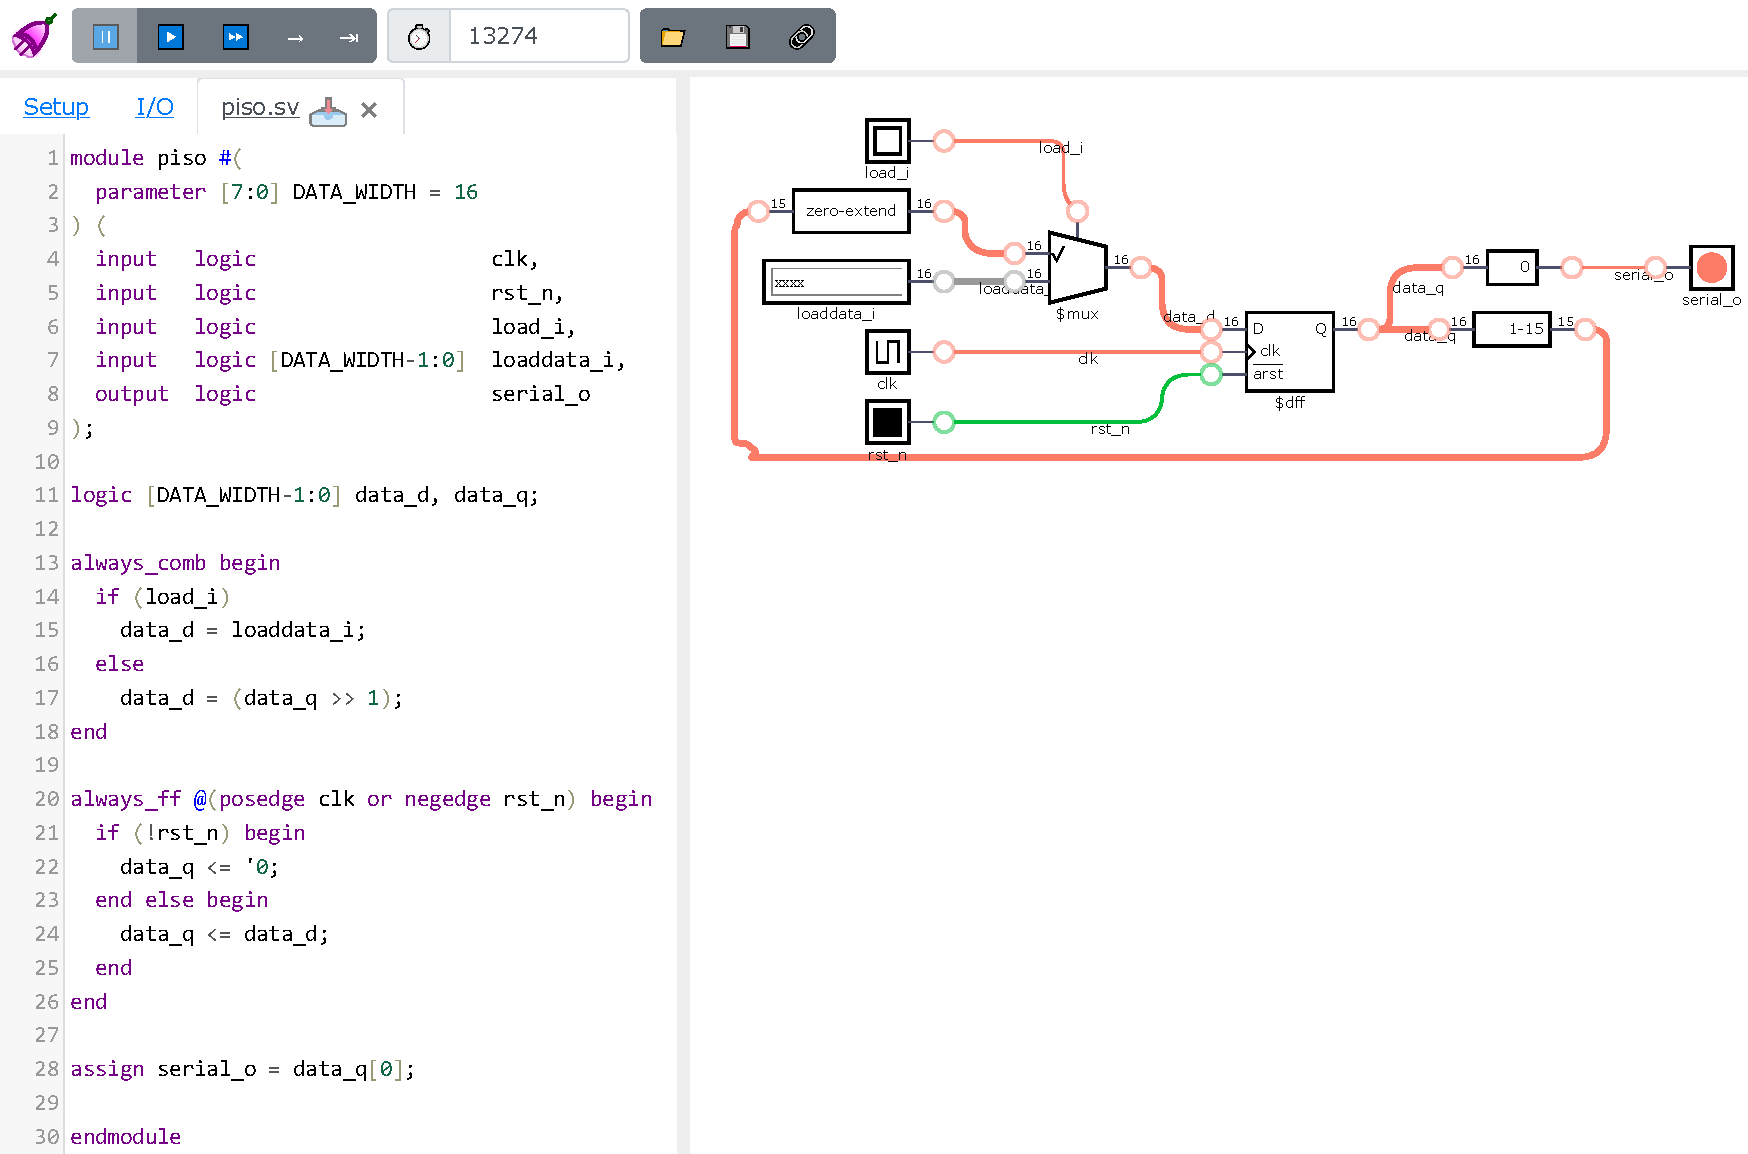
\includegraphics[width=\linewidth]{figures/digitaljs_online.pdf}
    \caption{Schematic for a Parallel-in Serial-out shift register generated by the netlist graph viewer DigitalJS Online \cite{DigitalJSOnline}}
    \label{fig:digitaljs_online}
\end{figure}


By using netlist graph viewers to provide a visual representation of the synthesis process, students can gain a deeper insight into how their high-level descriptions are transformed into hardware components.
DigitalJS Online \cite{DigitalJSOnline} stands as a notable example of such netlist graph viewers (see \autoref{fig:digitaljs_online}).
Through its zero-setup, interactive web interface, students can witness instant translation of their Verilog code into synthesized hardware, which encourages experimentation and rapid prototyping.
Additionally, its text editor runs automatic linting with Verilator, which gives incredibly helpful feedback if a syntax-related bad-practice is detected.
During a volunteer lecture for UCSB's IEEE student chapter, I taught Verilog concepts from DigitalJS Online's text editor, which seamlessly visualized the logic I was describing in my examples.
Also, as a TA for ECE 152A and 154B, I curated several assignments that challenged students to use DigitalJS Online to transform \mintinline{SystemVerilog}{for} loops and \mintinline{SystemVerilog}{if} statements into comprehensive, hand-drawn circuit diagrams.
Similarly, UC Santa Cruz Professor Dustin Richmond uses netlist graph viewers to teach best practices concerning \mintinline{SystemVerilog}{case} and \mintinline{SystemVerilog}{if} statements \cite{RichmondLatchUp}.
Plus, after enough exploration with netlist graph viewers, students can gain the ability to convert Verilog to schematics by hand.
By assigning homework and in-lecture exercises that prompt students to deduce hardware constructs from abstract Verilog syntax, their aptitude to understand both Verilog and synthesis will be significantly enhanced.

\FloatBarrier

\section{Enabling optimizations in netlist graph viewers creates complexity.}
\label{section:optimizations_in_netlist_graph_viewers}


\begin{figure}[t]
    \centering

    \subfloat[
        If any bits of \mintinline{systemverilog}{a} are set, then \mintinline{systemverilog}{out} is \mintinline{systemverilog}{1}.
    ]{
        \begin{minipage}{0.8\textwidth}
            \inputminted[frame=single]{systemverilog}{code/opt.svh}
        \end{minipage}
    }

    \subfloat[
        Vivado infers the code as one parallel LUT.
    ]{
        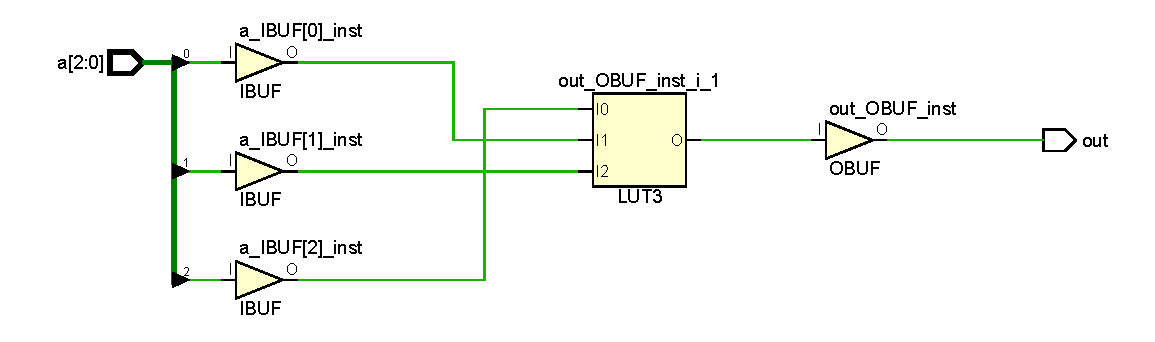
\includegraphics[width=0.9\linewidth]{figures/opt/vivado.pdf}
    }

    \subfloat[
        Yosys without optimizations enabled infers the code as a series of 2:1 MUXes.
    ]{
        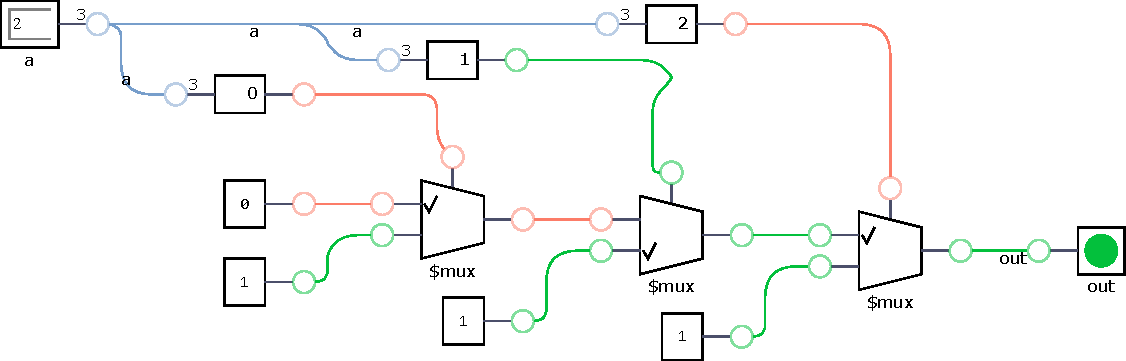
\includegraphics[width=0.7\linewidth]{figures/opt/yosys_noopt.pdf}
    }

    \subfloat[
        Yosys with optimizations enabled infers the code as one parallel OR gate.
    ]{
        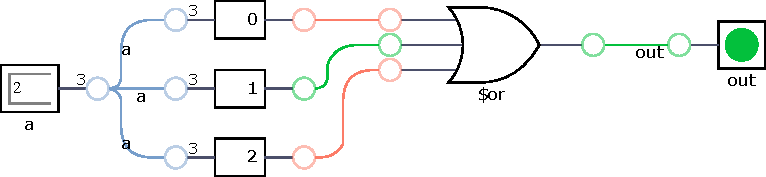
\includegraphics[width=0.7\linewidth]{figures/opt/yosys_opt.pdf}
    }

    \caption{Comparison of differences in synthesis.}
    \label{fig:opt}

\end{figure}


While synthesis tools may run their own specific optimizations \cite{1364.1-2005}, learning these intricacies are not critical, given the overall proficiency of available tools and the limited need for target-specific code optimization.
Instead, the primary focus should be on teaching students to write clear and transferable code, adhering to best practices covered in the class.
(This focus is also described in \autoref{section:leaderboard}).
While it is acceptable to encourage students to explore various tool and language features as illustrated in \autoref{fig:opt}, it is crucial to maintain a balance.
Experimentation can stimulate curiosity and self-directed learning, but there may be instances where netlist graph viewers create confusion rather than facilitate understanding.
For example, as students start working with larger designs, the chances are increased that a quietly-applied, tool-specific synthesis optimization will result in a netlist that, while valid, would take too much time to decipher and understand.
This may turn instructors away entirely from using netlist graph viewers due to the additional complexity that they cause.
However, I argue that they are still an essential resource for introducing Verilog, helping students transition from gate schematics to HDLs.
These tools serve as a foundation for students to build their intuition for synthesis, ultimately empowering them to undertake the more advanced design challenges.
Even if netlist graph viewers lose their effectiveness as designs get complex, they illustrate to students the vital connection between digital design concepts and Verilog concepts.

A similar example is providing simplified schematics of transistor implementations of digital gates to relate electrical engineering students to their prior knowledge of analog design.
Because transistor implementation specifics are largely unimportant due to the low demand for PDK designers, it is fine to simply introduce basic technologies such as pass-transistor logic instead of analyzing modern multi-finger FinFET CMOS designs.
But only after receiving \emph{some} connection to their prior experience with transistors will electrical engineering students feel comfortable working with gates.
Similarly, when introducing Verilog, netlist graph viewers can connect prior knowledge of digital elements to code syntax.
Much like electrical engineers need some familiarity with transistor-level gate implementations prior to diving into digital design, Verilog students greatly benefit from a basic understanding of the behavior of synthesis tools.

\FloatBarrier

\section{Teaching features that rely on inference is difficult but important.}
\label{section:inference_is_inconsistent}


\begin{figure}[t]
    \centering
    \frame{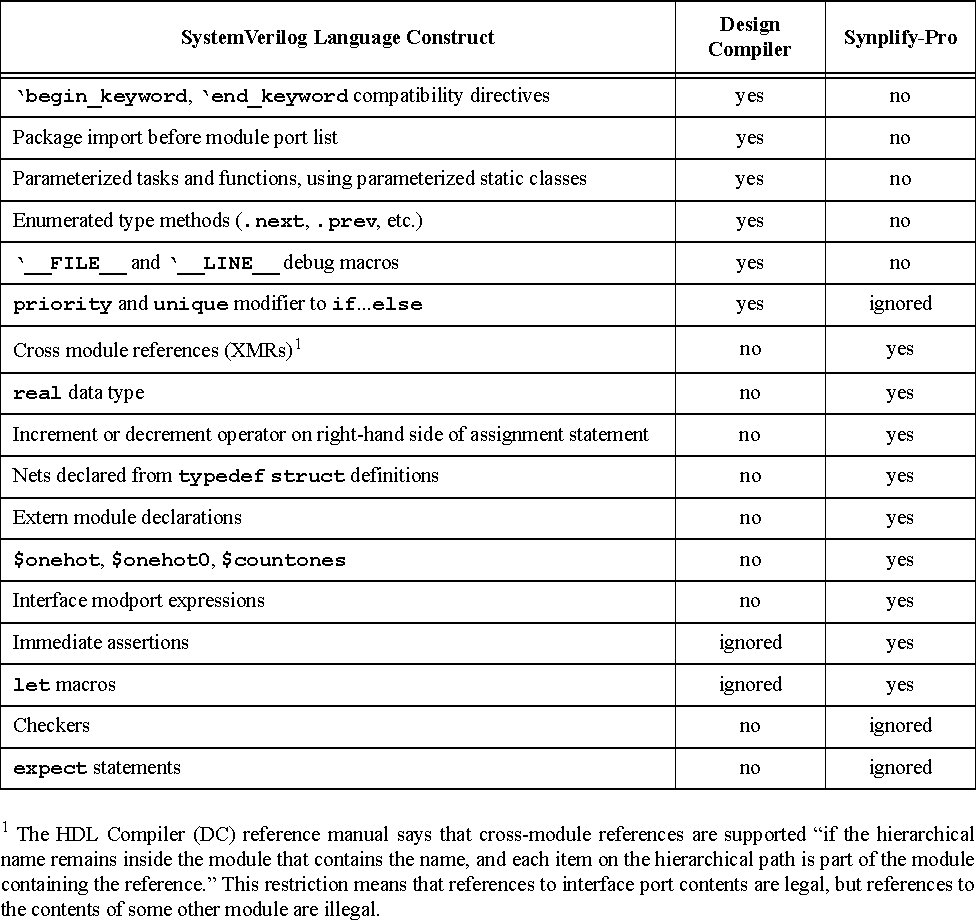
\includegraphics[width=\linewidth]{figures/dc_vs_synplify.pdf}}
    \caption{Differences in SystemVerilog Support in DC vs. Synplify-Pro from ``Synthesizing SystemVerilog: Busting the Myth that SystemVerilog is only for Verification''\cite{sutherland}}
    \label{fig:dc_vs_synplify}
\end{figure}


To promote uniformity among tools, IEEE standardized synthesis of Verilog 1364 features under the label \enquote{1364.1}.
However, there has been no official \enquote{1800.1} SystemVerilog synthesis standard to discuss the many new features that were added with SystemVerilog.
Many SystemVerilog IEEE 1800 features are not consistently synthesizable by popular synthesis tools, such as classes, interfaces, and dynamic arrays \cite{1800-2017, sutherland, sutherland:book}.
This may result from a SystemVerilog feature being subjectively similar to a prohibited feature in the IEEE 1364.1 standard, or may be due to insufficient tool development time.
For these reasons, support for many features is inconsistent across different open-source tools \cite{svtests}, and \autoref{fig:dc_vs_synplify} shows Synopsys' own tools have inconsistencies across each-other.
Since there is no official synthesis standard, style guides and linters have filled the role of unofficial documentation of SystemVerilog's synthesizable features to help engineers navigate the inconsistencies across different tools.
This is further discussed in \autoref{section:style_guides} and \autoref{chapter:autograders}.


\begin{figure}[t]
    \centering

    \subfloat[
        Using purely structural constructs to create MUXes can provide long and superfluous code.
    ]{
        \begin{minipage}{0.8\textwidth}
            \footnotesize
            \inputminted[frame=single]{systemverilog}{code/c-like/low.svh}
        \end{minipage}
    }

    \subfloat[
        Using C-like constructs such as a \mintinline{systemverilog}{function}, \mintinline{systemverilog}{if} statement, and \mintinline{systemverilog}{for} loop can provide much cleaner code.
    ]{
        \begin{minipage}{0.8\textwidth}
            \footnotesize
            \inputminted[frame=single]{systemverilog}{code/c-like/high.svh}
        \end{minipage}
    }

    \caption{Comparison of purely structural Verilog versus C-like Verilog. To demonstrate this comparison, provided are two different implementations of the Find First Set operation.}
    \label{fig:c-like}

\end{figure}


A reaction to the inconsistency and ambiguity in SystemVerilog synthesis may be to teach only obviously-synthesizable constructs such as continuous assignment (\mintinline{SystemVerilog}{assign}) and standard cell initialization, but that would neglect important language features that have become popular in industry designs.
Modern-day RTL engineers regularly use constructs such as procedural blocks, \mintinline{SystemVerilog}{for} loops, and \mintinline{SystemVerilog}{if} statements from Verilog; and \mintinline{SystemVerilog}{struct}, \mintinline{SystemVerilog}{union}, and \mintinline{SystemVerilog}{enum} constructs from SystemVerilog.
Similarly, in computer programming courses, once students understand the underlying mechanisms, it is common to allow use of standard library functions and data structures.
This philosophy should extend to the realm of SystemVerilog.
As long as the code adheres to linters and well-verified style guides, and students understand the resulting synthesis, higher-level syntax should be prioritized when it improves code clarity and structure, such as in \autoref{fig:c-like}.

\FloatBarrier

\section{HDLs can be abstractions for complex hardware concepts.}

With the full set of synthesizable features being utilized, Verilog can be a useful abstraction layer to better explain complex design concepts such as state machines, pipelining, and handshakes.
This parallels the use of abstraction in programming courses, where students often draft pseudocode to conceptualize algorithms before delving into detailed implementation.
Transferring this approach to digital design can promote a more rapid and comprehensive learning experience.
As long as students demonstrate a strong understanding of how Verilog can be synthesized, they will also have an understanding of the circuits needed to implement the complex design concepts.
An example of this in practice was when UCSB ECE 154B students were assigned my \enquote{Labs with CVA6} Cache Lab, where students were expected to implement a doubly-linked-list to execute a least-recently-used (LRU) replacement policy.
With the helpful abstraction layer of structs, \mintinline{SystemVerilog}{for} loops, and \mintinline{SystemVerilog}{if} statements, (as seen in \autoref{fig:cache_lab}), students were able to demonstrate a high-level understanding of the LRU algorithm while also understanding the low-level hardware that was generated.


\chapter{Best Resources for Learning Synthesizable SystemVerilog}
\label{chapter:resources}

When writing synthesizable SystemVerilog, not all features present in the IEEE 1800 specification can be utilized, as synthesis tools support only a subset of these features. Unfortunately, many educational resources for Verilog and SystemVerilog fail to document which features are synthesizable and which are for verification only. To combat this ambiguity, a curated set of resources dedicated to synthesis should be prioritized when giving students additional materials for outside the classroom.

\section{Stuart Sutherland's synthesis guide is most valuable.}

\enquote{Synthesizing SystemVerilog: Busting the Myth that SystemVerilog is only for Verification} by Stuart Sutherland and Don Mills acts as a comprehensive list of synthesizable SystemVerilog features. Despite the absence of an official SystemVerilog synthesis standard, this paper gives valuable insight into synthesizable language features, emphasizing their practical application into modern hardware designs. Sutherland and Mills surveyed the Synopsys tools Design Compiler and Synplify-Pro to trace the evolution of Verilog-1984 though SystemVerilog-2009 as a comprehensive hardware design and verification language. To assist those working on \enquote{Labs with CVA6}, I composed a summary of Sutherland's synthesis guide \cite{labsWithCVA6}. Since then, I have shared this summary with dozens of students looking to improve their understanding of synthesizable Verilog. Providing both Sutherland's guide and my summary ensures that students receive a strong introduction to synthesizable Verilog syntax and best practices.

\section{Style guides and linters record synthesizable features and best-practices.}
\label{section:style_guides}

Even while avoiding commonly unsynthesizable SystemVerilog features, design tools are infamous for misinterpreting syntax and often providing little or misleading information on errors. Therefore, using linters and well-verified style guides is crucial in ensuring that an RTL implementation will work on an assortment of tools. As mentioned in \autoref{chapter:digital_design}, style guides and linters help direct engineers away from ambiguous or poorly-supported language features, and towards syntax and features that are verified to tape-out chips successfully. By introducing Verilog alongside an exhaustive style guide, and providing test flows with linting, students can feel much more confident exploring new language features.

The lowRISC Style Guide discusses many best-practices of language features such as the alias statement, automatic scopes, package imports, and floating begin-end blocks \cite{lowRISCstyleguides}. The Bespoke Silicon Group Style Guide is also strong due to its discussion of structures, enumerations, and memories \cite{BSGstyleguide}. There are also style guides published by tool manufacturers that show how to infer different types of logic \cite{Xilinxstyleguide, Intelstyleguide, Latticestyleguide}. There are many style guides available; see \autoref{appx:style_guides} for a(n incomplete) list. Personally, I teach the lowRISC style guide because of its thorough explanations, because of the clarity in \mintinline{systemverilog}{_d} and \mintinline{systemverilog}{_q} as suffixes for register inputs and outputs, and to match the \enquote{Labs with CVA6} project (as described in \autoref{chapter:labs_with_cva6}).

Linters such as Verible \cite{veribleGitHub}, Verilator \cite{verilatorGitHub}, and svlint \cite{svlintGitHub} are all popular in design flows. Each are configurable to warn on or forbid specific language features, and many open-source projects choose to lint with more than one of these tools. For example, Verible is known for its auto-formatting capabilities; Verilator is powerful enough to warn on multidriven signals and accidental latches in \mintinline{systemverilog}{always_comb} blocks; and Svlint is unique for its ability to verify complex whitespace layouts and enforce custom net naming styles. Each have their purpose and should be used on student submissions to ensure best-practices are enforced.

\section{Verilog tutorial websites should be treated cautiously.}

It is important to stress the importance of following the provided style guides for Verilog syntax over some of the most popular Verilog tutorial websites, such as ASIC World, Chipverify, and Nandland. Despite the user-friendly approach adopted by these websites, which mirror renowned programming tutorial platforms such as GeekforGeeks, Verilog tutorial websites often propagate misguided advice for novice hardware developers. While style-guides can act as a reference to well-verified practices for beginners and professionals alike, tutorial websites do not always teach current-day, synthesizable design syntax that is compatible with a multitude of tools. Only if students maintain adherence to the instructor-specified style-guides and the subset of synthesizable features, then tutorial websites can be used as resources.


\begin{figure}[t]
    \centering
    \inputminted[frame=single]{systemverilog}{code/always_ff.svh}
    \caption{Potentially confusing behaviors of \mintinline{systemverilog}{always_ff} blocks}
    \label{fig:always_ff}
\end{figure}


\begin{figure}[t]
    \centering
    \frame{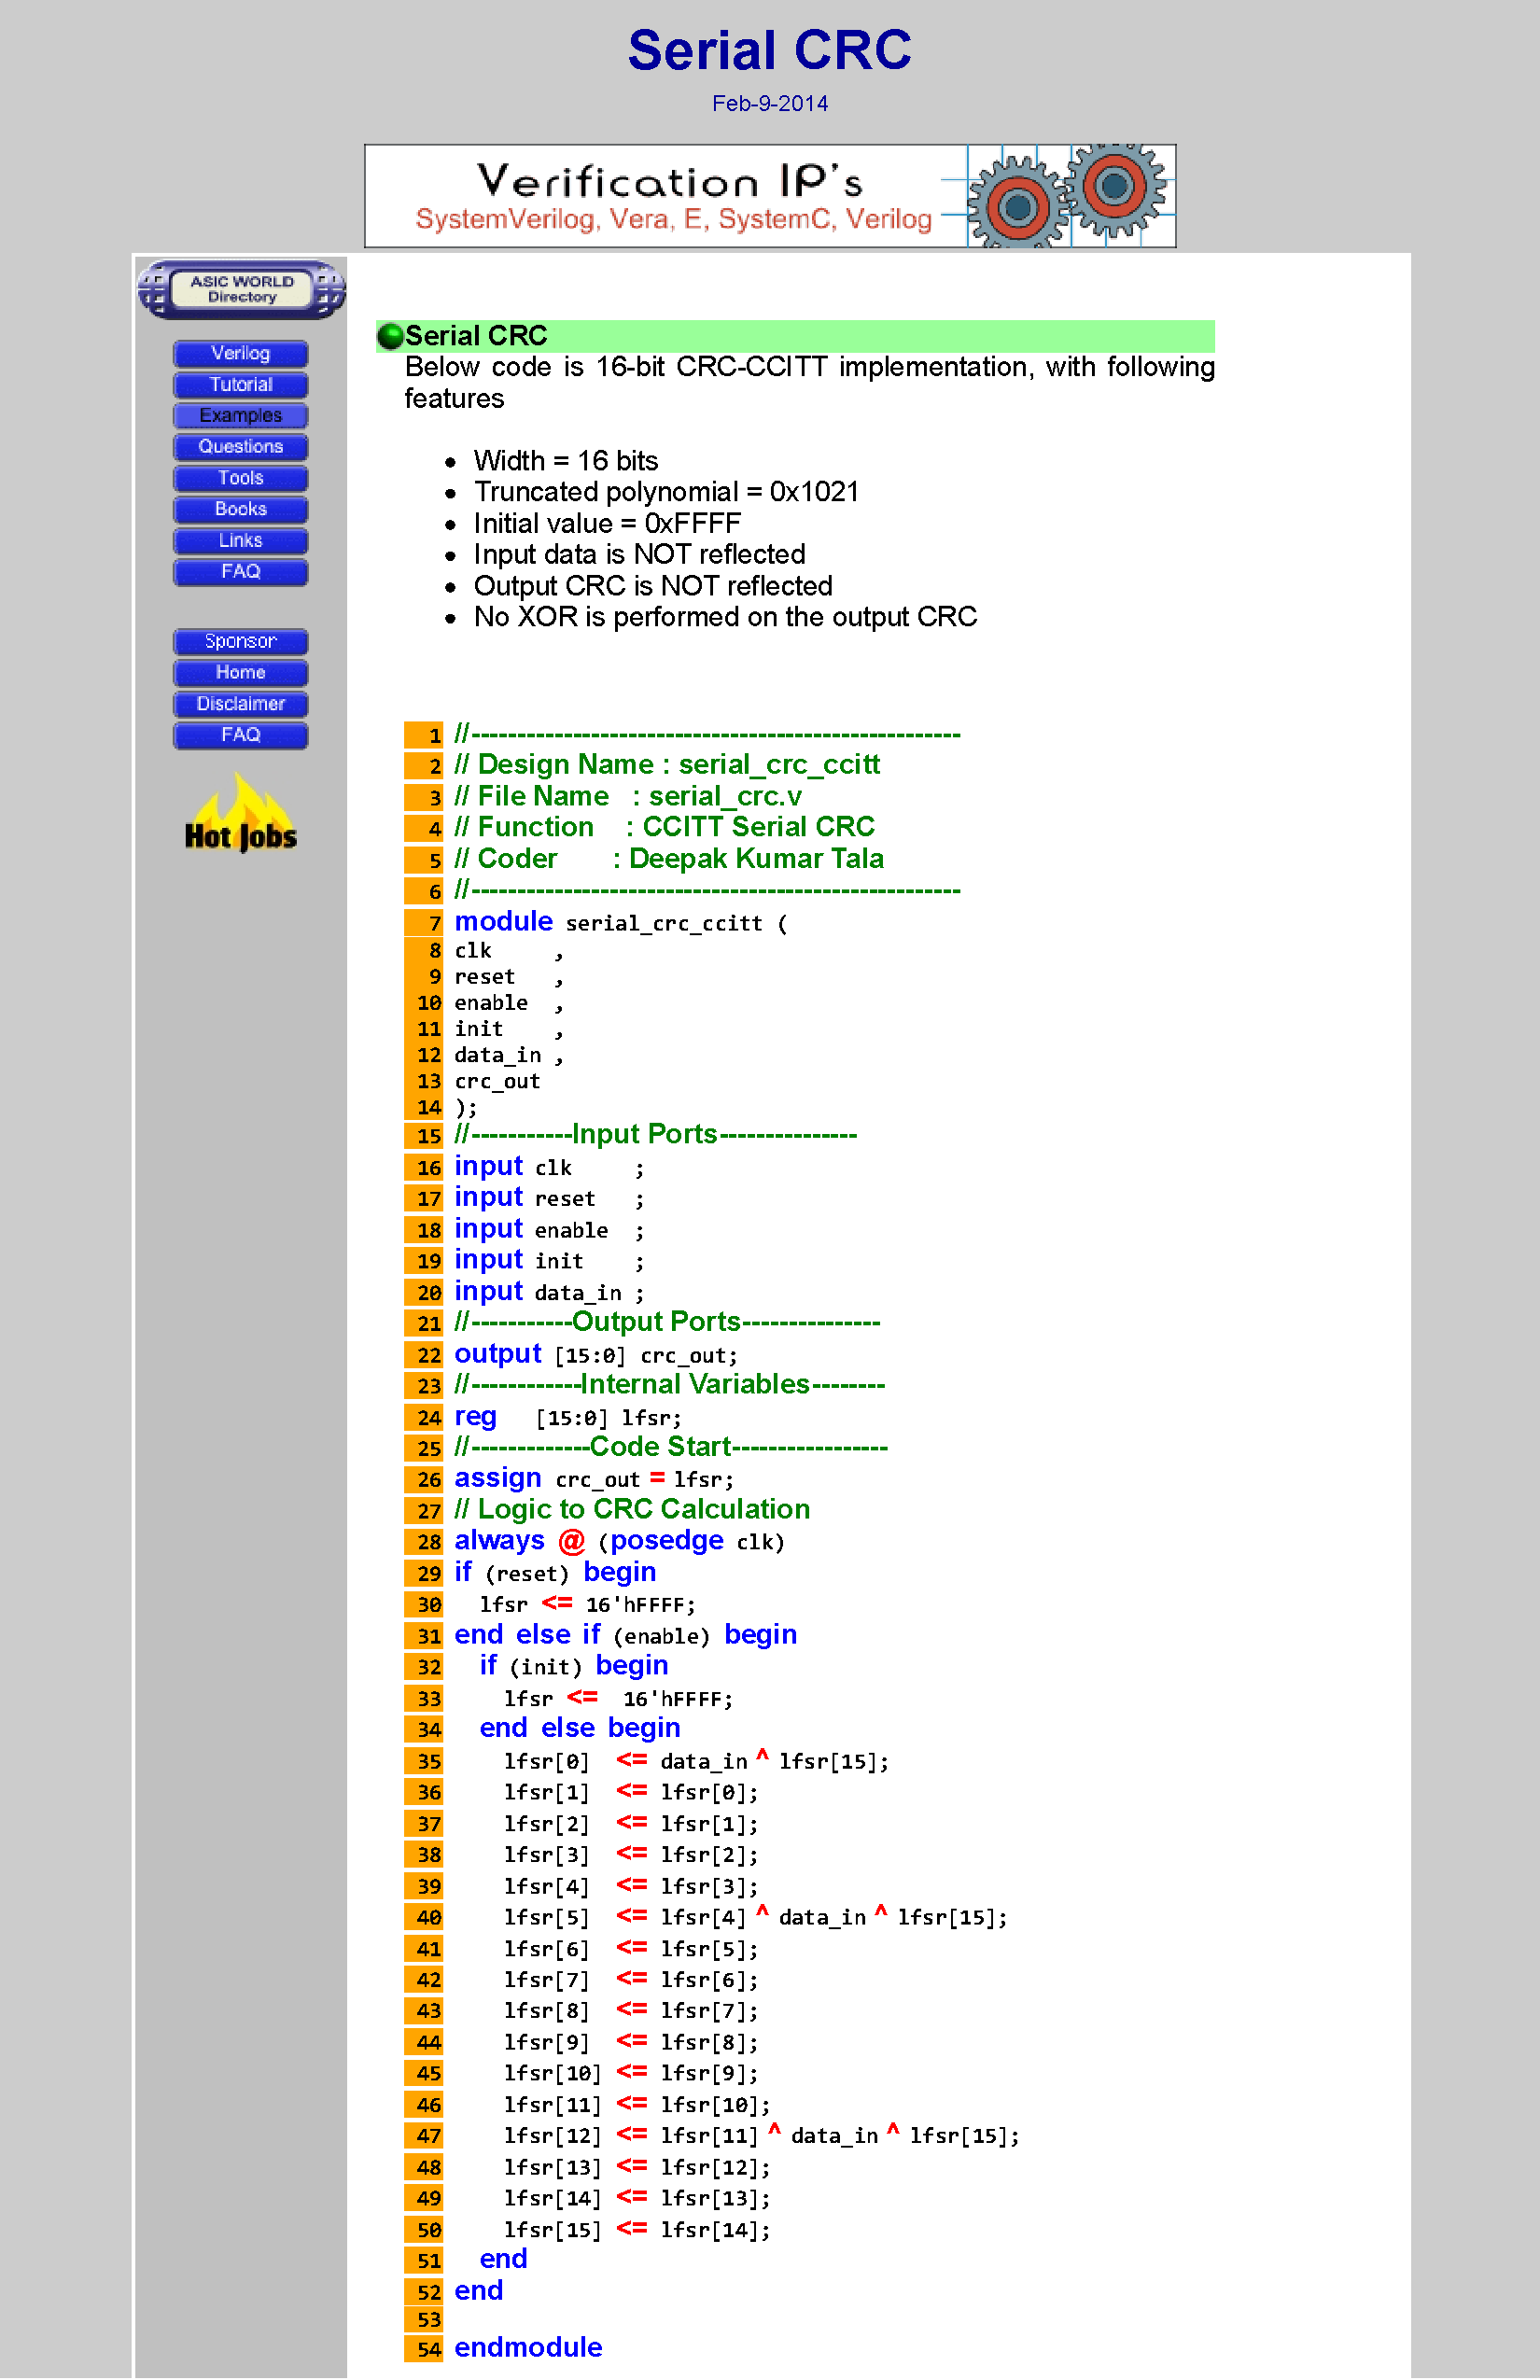
\includegraphics[width=\textwidth,height=0.9\textheight,keepaspectratio]{media/asicworld.pdf}}
    \caption{This is an example provided by ASIC World that encourages bad design practices \cite{asicworld}}
    \label{fig:asicworld}
\end{figure}


For example, while a TA for ECE 152A, 154A, and 154B, the most prevalent misinformation they encouraged in students was to put combinational logic inside of \mintinline{systemverilog}{always_ff} blocks. (See \autoref{fig:asicworld}). The lowRISC Style Guide, the BSG SystemVerilog Coding Standards, and the IEEE 1364.1-2005 Verilog Synthesis Standard all recommend only putting resets, sets, and enables in \mintinline{systemverilog}{always_ff} blocks \cite{lowRISCstyleguides, BSGstyleguide, 1364.1-2005}. Unnecessarily large \mintinline{systemverilog}{always_ff} blocks are prone to bugs because \mintinline{systemverilog}{always_ff} blocks don't offer warnings on unhandled code paths, blocking and nonblocking-assignment mismatches can lead to undefined behavior, and synthesis tools may incorrectly infer the incorrect type of flip-flop. (See \autoref{fig:always_ff}). In my experience teaching SystemVerilog, whenever a student asked for help solving a bug, but followed this design practice, I immediately asked them to separate the block into an \mintinline{systemverilog}{always_comb} and \mintinline{systemverilog}{always_ff}. Over half the time, that simple refactor incidentally fixed the student's bug.

\FloatBarrier

\section{ChipDev.io can be used to practice Verilog (if used effectively).}


\begin{figure}[t]
    \centering
    \frame{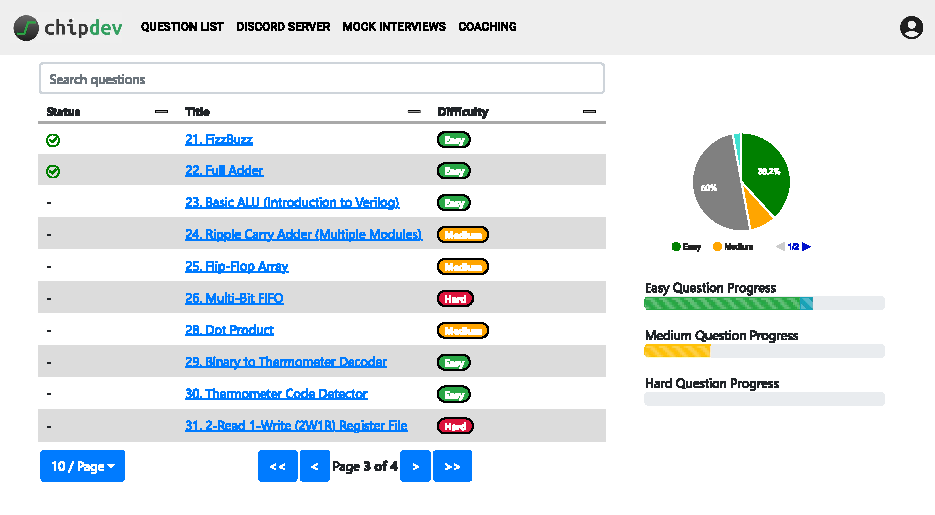
\includegraphics[width=0.7\linewidth]{media/chipdev_questions.pdf}}
    \caption{An example of questions that ChipDev offers. \cite{ChipDev}}
    \label{fig:chipdev_questions}
\end{figure}


\begin{figure}[t]
    \centering
    \frame{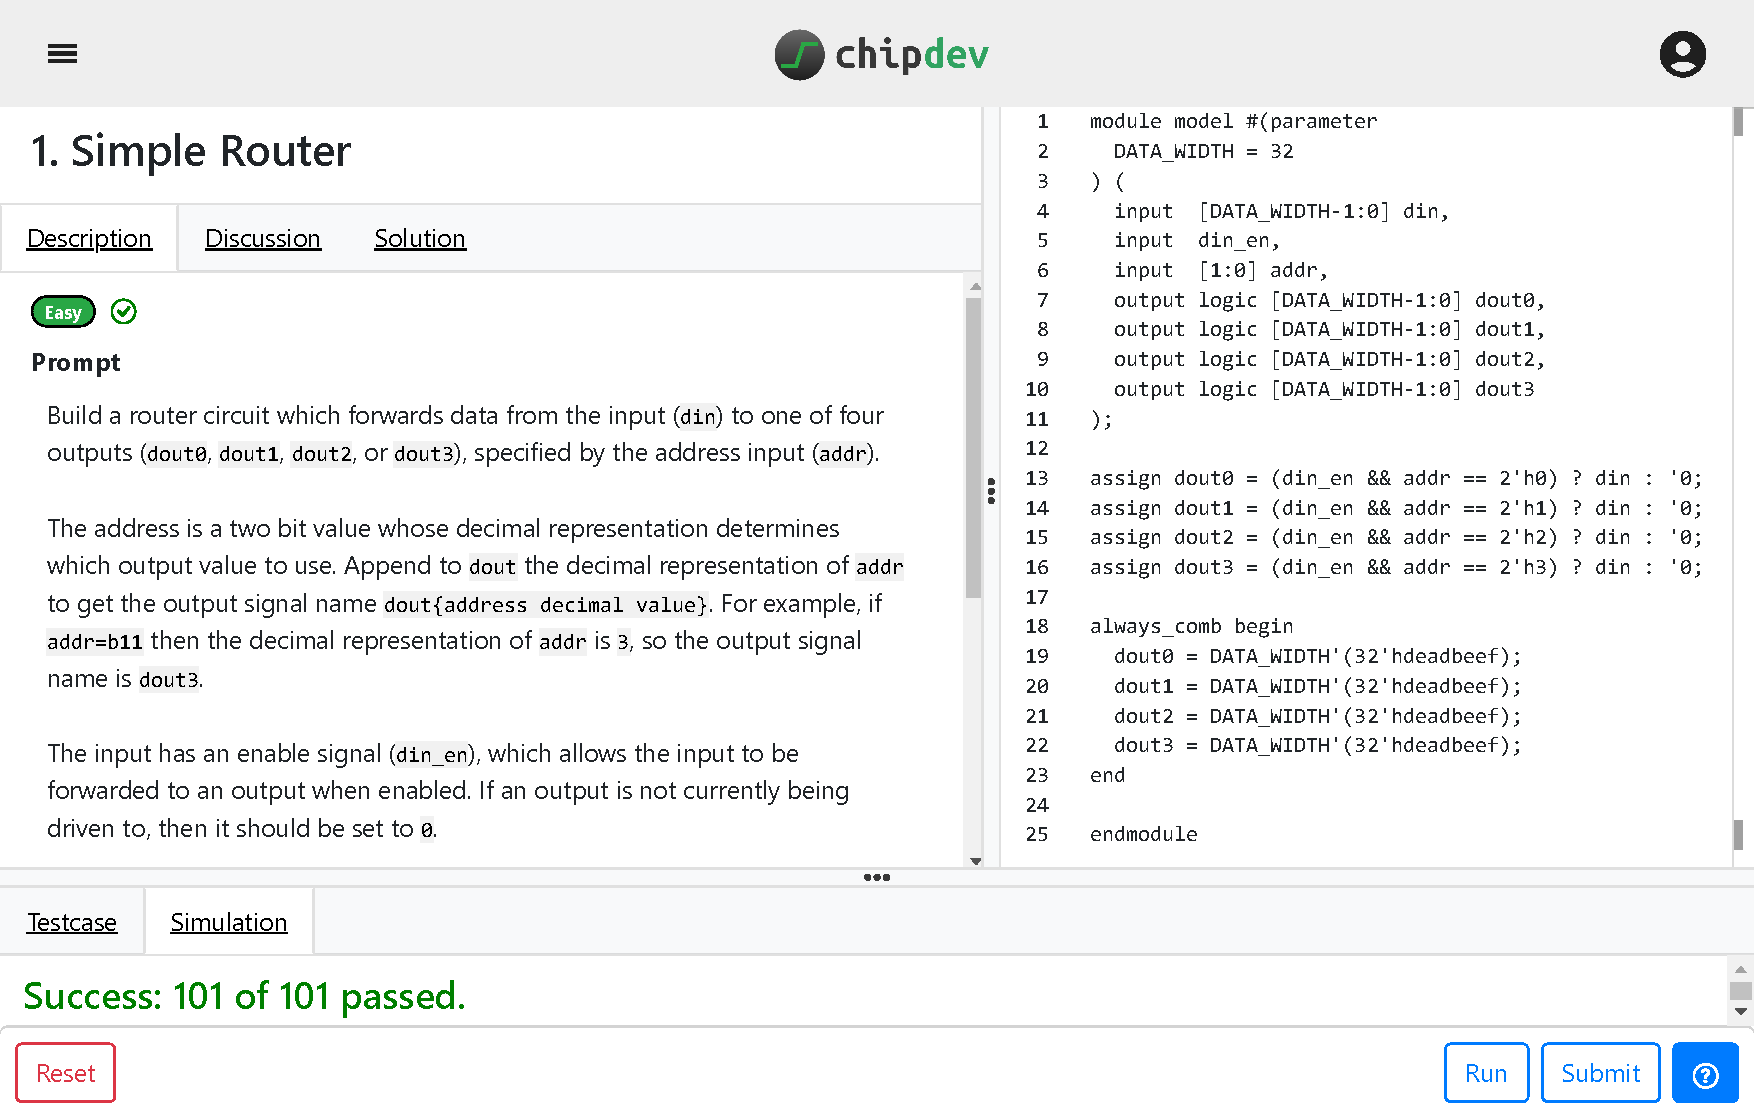
\includegraphics[width=0.9\linewidth]{figures/chipdev_hack.pdf}}
    \caption{This example shows ChipDev \cite{ChipDev} incorrectly accepting this submission despite a potential mismatch between simulation and synthesis. For example, Verilator will override the \mintinline{systemverilog}{always_comb} with the \mintinline{systemverilog}{assign}, but Yosys will override the \mintinline{systemverilog}{assign} with the \mintinline{systemverilog}{always_comb}. This could be corrected if ChipDev chooses to incorporate a similar verification flow to what is outlined in \autoref{section:complex_tool_setups}.}
    \label{fig:chipdev_hack}
\end{figure}


The final resource I like to share with students is ChipDev.io, which offers an online collection of popular Verilog questions, paired with an online IDE and testbench. The 30+ questions range from implementing a shift register to designing an ALU; (see \autoref{fig:chipdev_questions}). If students are looking for lots of practice questions as job interview preparation or for general practice, I always recommend ChipDev. However, ChipDev does not run gate-level simulation or logical equivalence checks, so bad submissions may be incorrectly rewarded; (see \autoref{fig:chipdev_hack}). Plus, after speaking with the ChipDev team, they notified me that synthesis was not on their priority list. Therefore, I strongly urge students to verify their answers with DigitalJS Online or other synthesis tools before feeling they have a mastery over any question.


\chapter{Teaching Code Scalability and Development Practices}
\label{chapter:scalability}

Aside from ensuring that student code follows best-practices and correctly synthesizes, an equally important skill to teach students is how to efficiently work on large-scale projects. As the number of transistors on an integrated circuit has increased, the scale of Verilog designs has also drastically increased. At Intel, the SoC that my team was verifying had over 500 Verilog source files in the design. Similarly, one of the most popular RISC-V cores, CVA6, is written in nearly 17,000 lines of code \cite{cva6}. Ensuring seamless development and limiting the number of bugs within these colossal codebases requires strong project management skills. This is achieved by automatic regression, consistent coding styles, and employing version control. In more advanced Verilog courses such as Computer Architecture or SoC design, I argue that teaching code scalability is often just as important as teaching microarchitecture implementation methods.

\section{SystemVerilog offers many features to aid in code organization.}


\begin{figure}[t]
    \centering
    \small
    \inputminted[frame=single]{systemverilog}{code/ece152a_pkg.sv}
    \caption{This is a SystemVerilog package that was provided to ECE 152A students to aid in their implementation of a 1965 Ford Thunderbird taillight state-machine.}
    \label{fig:ece152a_pkg}
\end{figure}


Features such as packages, structs, and parameters are incredibly popular in large-scale SystemVerilog projects. And although IEEE 1364 Verilog does not support packages and structs, many RTL designers have found workarounds with \mintinline{systemverilog}{`include} files and functions. \cite{lowRISCstyleguides, zachjssv2vGitHub} These features may not be \emph{required} to implement hardware algorithms such as instruction decoding and serial interfaces, but are still extremely prevalent in well-organized, large-scale Verilog designs. In ECE 152A, ECE 154A, and ECE 154B, we were sure to teach students to apply these code organization strategies. See \autoref{fig:ece152a_pkg}.

\section{Version control should be used in Verilog designs.}

Aside from code structure, a cornerstone of modern software development is version control. Intel, numerous other companies, and most RISC-V projects extensively rely on Git and GitHub for version management. Moreover, Git submodules and subtrees provide an elegant solution for integrating IP blocks into designs seamlessly, enhancing reusability and collaboration. Plus, allowing students to post code they've written themselves to GitHub is a great way to aid them in creating an online portfolio for themselves. In ECE 154B, students practiced using Git and GitHub to explore open-source projects, collaborate with peers, add open-source cores as submodules, and more. While software might not be the core focus for some students, being able to work with it efficiently and professionally is still extremely valuable. Because of the invaluable aid Git offers in code quality, and its extreme prevalence in all software development, it is an invaluable hard-skill for all engineers.

\section{SystemVerilog assertions and in-module verification are important.}

The final design strategy for promoting code scalability is to promote in-module verification. Waveform viewers are incredibly powerful and useful tools, but work best when supplemented with \mintinline{systemverilog}{$display} statements that have already identified where and when a simulation error occurred. Most SystemVerilog in industry designs is full of self-verifying modules by use of SystemVerilog assertions (SVA) and Universal Verification Methodology (UVM). Note that as of 9/10/23, since there is poor SVA and UVM support in open-source tools, projects may need to use \mintinline{systemverilog}{`ifdef} macros to disable UVM and SVA calls on a per-tool basis, may need to limit themselves to the subset of supported features, or may need to resort to a basic \mintinline{systemverilog}{always} blocks instead. But no matter the specific implementation, in-module verification is a valuable design practice to teach students. In ECE 152A, ECE 154A, and ECE 154B, students were often required to design modules that incorporated simulation-only logic to test basic functionality. By adopting these universal standards, Verilog education becomes better aligned with real-world methodologies for enhanced scalability and proficiency.


\chapter{Autograders}
\label{chapter:autograders}

The incorporation of autograders within Verilog/SystemVerilog education is arguably the most valuable aspect of RTL education. These tools, particularly exemplified by platforms like Gradescope, can introduce a dynamic and interactive dimension to the learning process, revolutionizing the way students engage with Verilog concepts. Leveraging custom docker containers and custom Bash scripts, Gradescope's autograders easily facilitate Verilog testbench simulations, strict linting, synthesis, gate-level simulation, and more, yielding insights and feedback on various aspects of student submissions. However, managing software licenses on autograder servers can be a hassle, so all these functionalities are often best deployed with open-source tools. In the context of UCSB's ECE 152A, 154A, and 154B courses, students responded extremely positively to autograders, visibly enhancing their mastery over synthesizable Verilog.

\section{Autograders offer instant, high-quality feedback.}

Students are empowered to submit their code multiple times, enabling them to refine their solutions and learn from their mistakes in real time. This back-and-forth approach ensures that students can practice a Verilog concept and receive as much help as they need until they pass all the instructor-defined tests. In the autograders that I set up, it is worth noting that a significant majority of students eventually achieve a 100\% score by the assignment deadline. Therefore, autograders fall under the educational approach known as \enquote{Ungrading,} where the emphasis shifts strongly toward providing valuable feedback over assigning traditional grades. This phenomenon essentially transforms the grading system into a confidence-building mechanism rather than a competitive ranking system. Ungrading has been shown to help students by reducing stress, inspiring creativity, and encouraging healthy risk taking. \cite{kohn:book, blum:article} However, arguably Ungrading's largest downside is that the instructor may not have time to provide personalized feedback to all students. Fortunately, an intrinsic attribute of software, (such as HDL implementations), is that code quality and correctness can be run with automatic, subjective computer algorithms. Therefore, by implementing autograders, Verilog educators can easily tap into this pedagogical insight, offering students a more effective way to grasp digital design principles.

\section{Autograders can run remotely without complex local-setup.}
\label{section:complex_tool_setups}

When instructing students on crafting Verilog code that maintains accurate synthesizability across various platforms, it is essential to follow the industry standard of verifying a design with a wide selection of tools. Autograders streamline this process, making it accessible and efficient for students to perform comprehensive testing without the need for local installation. For example, the autograders that I created for ECE 152A, 154A, and 154B would consistently use anywhere from 6 to 10 different tools, sometimes requiring complex installation and setup procedures. Expecting students to complete these setup procedures is often tedious and counterproductive. Therefore, simply giving students access to a fully prepared autograder can remove the setup barrier completely.

As mentioned, an autograder test suite that closely mirrors industry quality should follow all the verification steps demonstrated in \autoref{fig:asic_flow}. First, it is important to run behavioral simulations with multiple tools such as Icarus, which supports propagation of unknown (\mintinline{SystemVerilog}{x}) values, and simulation with Verilator, which has stronger restrictions on bad syntax. Only by passing simulations with both tools should the autograder grant full points. Furthermore, code linters such as Verilator and Verible can ensure adherence to essential coding standards and practices, checking for issues like latches in \mintinline{SystemVerilog}{always_comb} blocks, correct use of blocking and non-blocking assignments, net-width discrepancies, and more. Considering that the frontends of tools do not always offer helpful warnings, this detailed syntax checking from Verilator and Verible is invaluable for students when fixing otherwise cryptic issues. Then, to deploy SystemVerilog synthesis with open-source tools, Yosys and Nextpnr must be paired with a frontend such as Surelog or zachjs/sv2v. The Yosys synthesis and Nextpnr layout process can verify if students are using too many logic cells, if their design is too slow, or if their design infers prohibited logic cells. As a final post-synthesis step, Icarus can be run one final time on the Yosys output to initiate a gate-level simulation (GLS) with unknown value propagation, and Yosys EQY can be run to perform logical equivalence checking (LEC). All of these features\footnote{Inclusion of LEC with EQY into an autograder remains outstanding due to time constraints during the project's development.} have been successfully implemented in autograders for ECE 152A, 154A, and 154B.

\section{\enquote{For-fun} leaderboards can excite and inspire students.}
\label{section:leaderboard}


\begin{figure}[t]
    \centering
    \frame{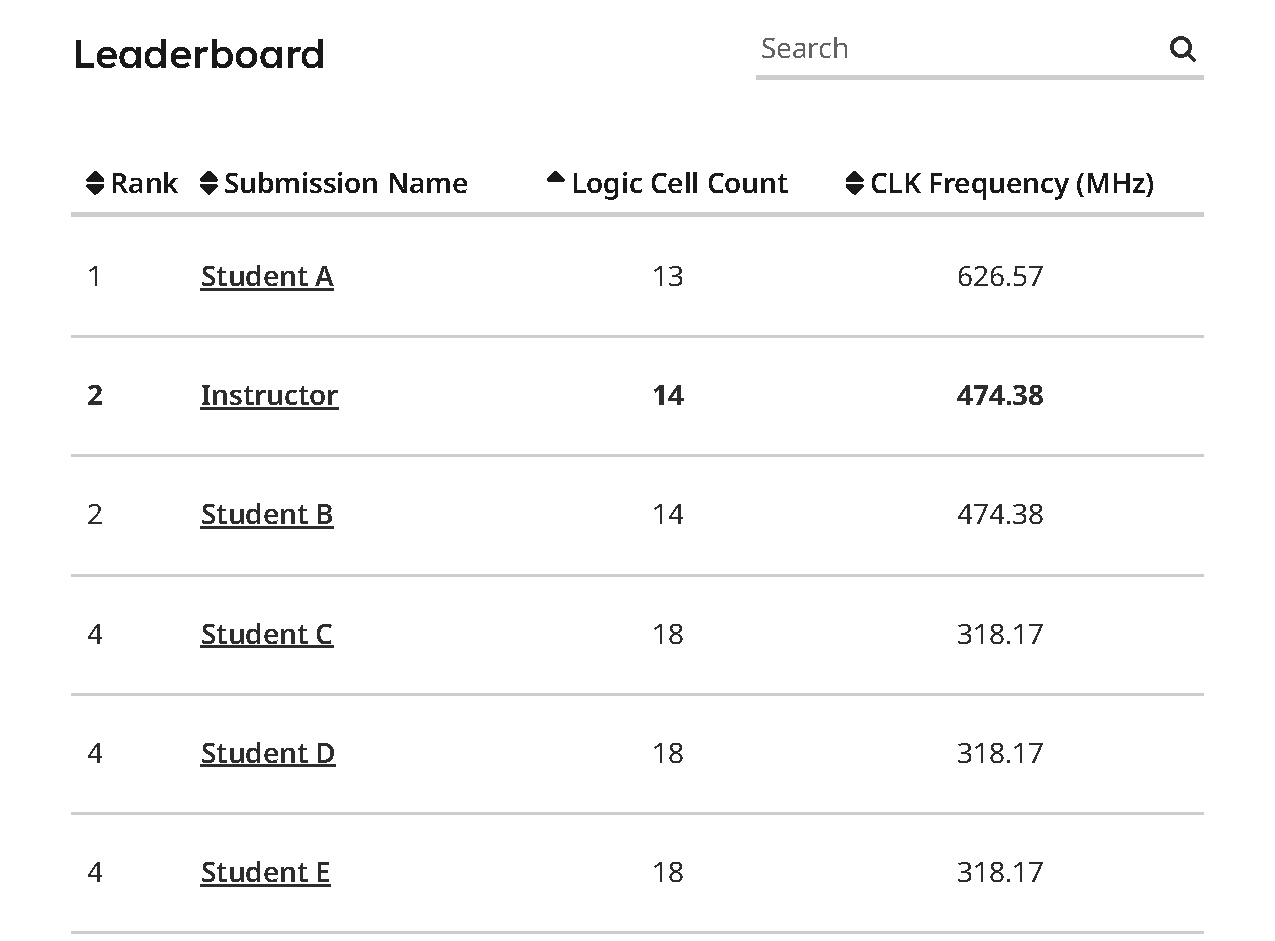
\includegraphics[width=0.8\linewidth]{media/graphics/leaderboard.pdf}}
    \caption[
        Gradescope Leaderboard
    ]{
        Example of a Gradescope leaderboard for a counter lab (same lab as in \autoref{fig:unreadable_opt}).
        Student designs were ranked on cell usage and maximum frequency as calculated by Yosys and Nextpnr-ice40.
        (Student names have been obfuscated for privacy reasons).
    }
    \label{fig:leaderboard}
\end{figure}


\begin{figure}[t]
    \centering
    \inputminted[frame=single]{systemverilog}{code/unreadable_opt.svh}
    \caption{Student drastically reduced readability and transferability in order to save 1 logic cell over the teacher solution.}
    \label{fig:unreadable_opt}
\end{figure}


Aside from a grade assigned by the autograder, another form of feedback can be provided through a class leaderboard. Students can see how their submission compares to the rest of the class on statistics such as logic cell usage, max clock frequency, or branch predictor hit percentage (see \autoref{fig:leaderboard}). Since the leaderboards in ECE 152A and 154B did not count towards any points, students really enjoyed seeing how each of their designs compared to their peers' designs, then would try to beat their friends for bragging rights. Because of this, I added leaderboards to every assignment that I could. However, it is important to clarify to students that code readability should be prioritized over moving up in the leaderboard by saving 1-2 logic cells. However, because autograders running purely open-source tools must only rely on Yosys and ABC for synthesis, students may be incorrectly rewarded for submissions that are not well-optimized for other more prevalent synthesis tools such as Design Compiler or Vivado (similar to \autoref{section:optimizations_in_netlist_graph_viewers}). This was a rare edge case that only visibly affected 1 submission (\autoref{fig:unreadable_opt}) across the 600+ leaderboard submissions I saw, but it is still important to monitor in students. Overall, creating assignment leaderboards was a great way to increase student enthusiasm without bringing additional stress or responsibilities.

\section{Autograders can foster community and collaboration.}

In ECE 152A, students discussed their challenges, insights, and strategies with peers, creating a collective learning environment. Since each student had a clear goal of \enquote{passing all the tests}, we saw students combine strategies and knowledge with confidence. Plus, ungraded leaderboards offered a fun but optional way for students to collaborate in friendly competitions. Communal engagement not only strengthens individual understanding, but also enriches the overall learning ecosystem. By integrating autograders, students experience a much more positive learning environment while still being provided critical skills and insights for their future engineering endeavors.


\chapter{Labs with CVA6 Project}
\label{chapter:labs_with_cva6}


\begin{figure}[t]
    \centering
    \frame{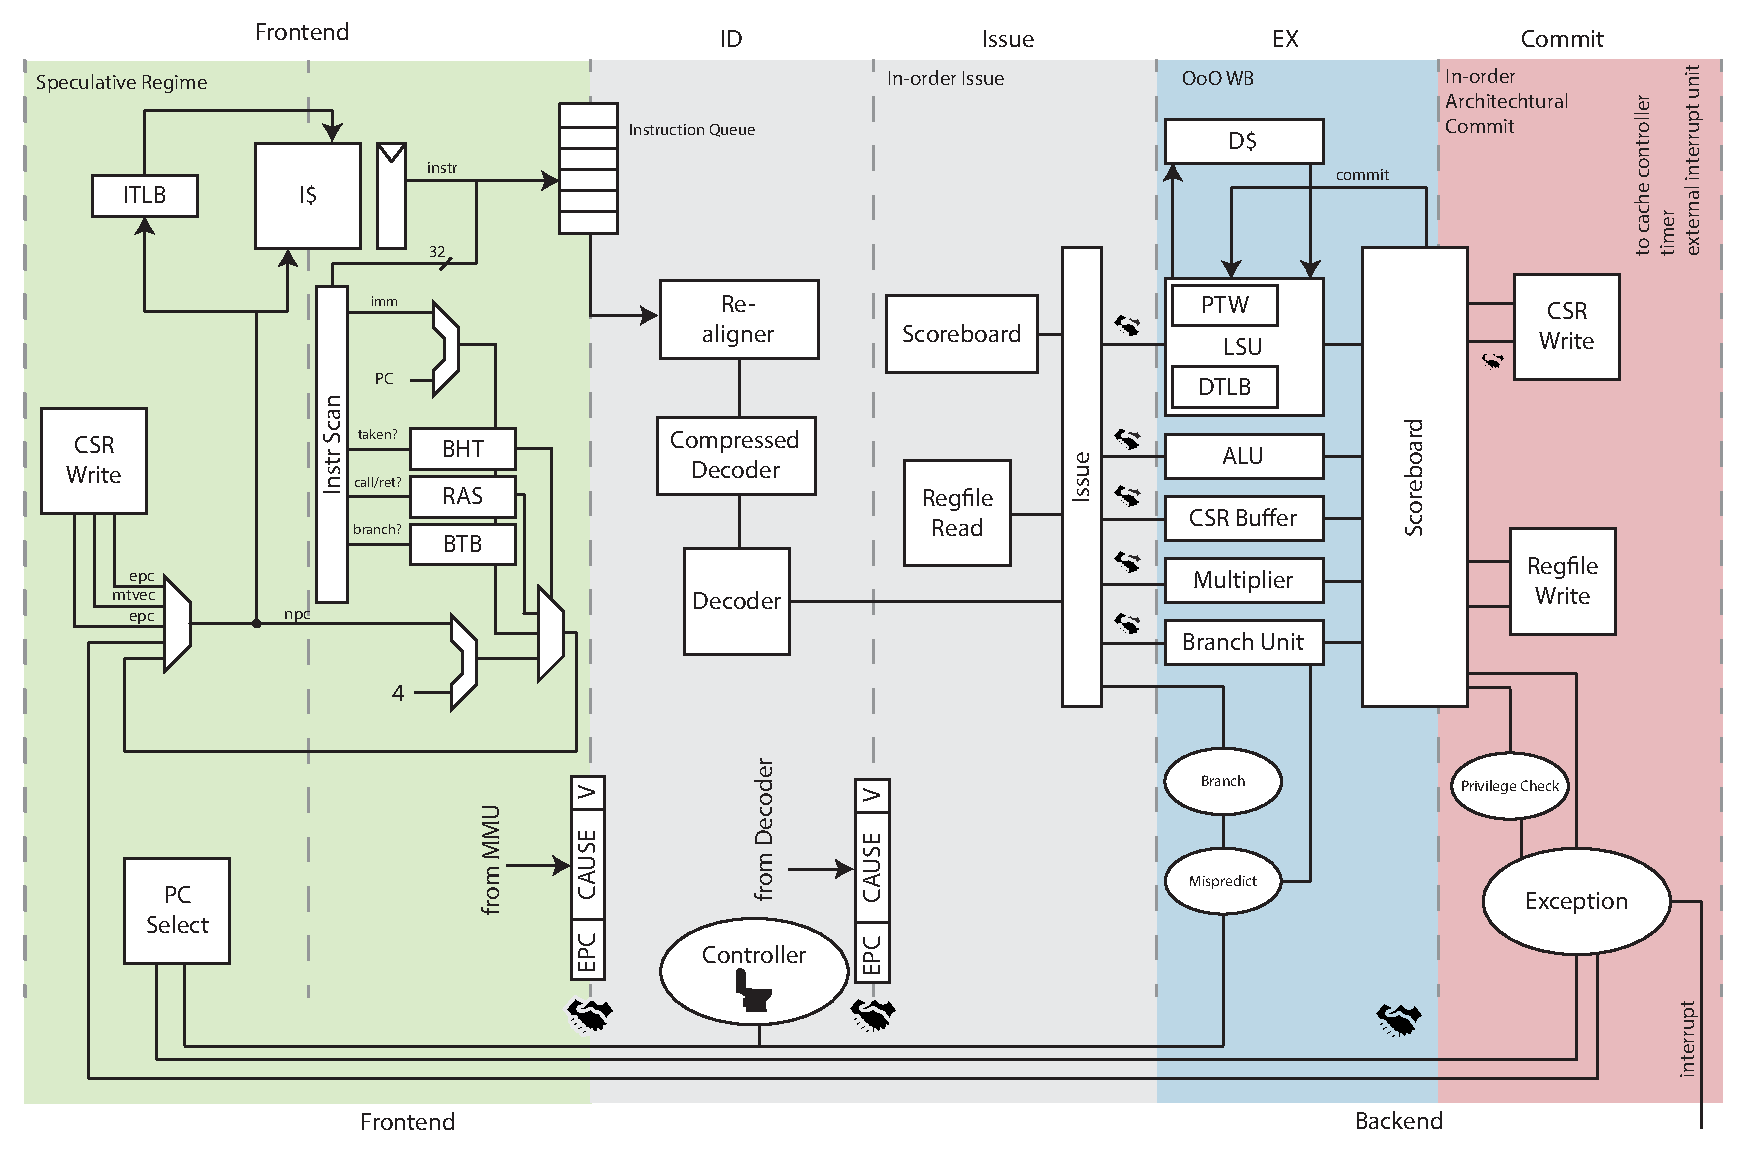
\includegraphics[width=0.7\linewidth]{media/cva6_overview.pdf}}
    \caption{CVA6 Block Diagram \cite{cva6}}
    \label{fig:cva6_overview}
\end{figure}


Standing as a culmination of all the Verilog education philosophies described in this thesis is a set of assignments I designed under the project label ``Labs with CVA6''. By drawing on my experiences from my time at Intel, my contributions to open-source projects, and interactions with industry contacts, I wrote four labs that aimed to give students practical experience with advanced computer architecture concepts. Each lab is centered around the fully featured RISC-V core CVA6, which is perfect for advanced architecture education due to its 6-stage pipeline, dynamic branch predictor, L1 cache, scoreboard unit, and virtual memory support (\autoref{fig:cva6_overview}). The labs presented students with a unique chance to engage with a fully-featured and transparent RISC-V core. This hands-on interaction facilitated a deeper comprehension of important architectural principles while also enhancing their ability to work with large and complex SystemVerilog designs. These labs are available for free under the BSD-3-Clause license \cite{labsWithCVA6}.

\FloatBarrier

\section{These labs provide hands-on exploration of architectural concepts.}


\begin{figure}[t]
    \centering
    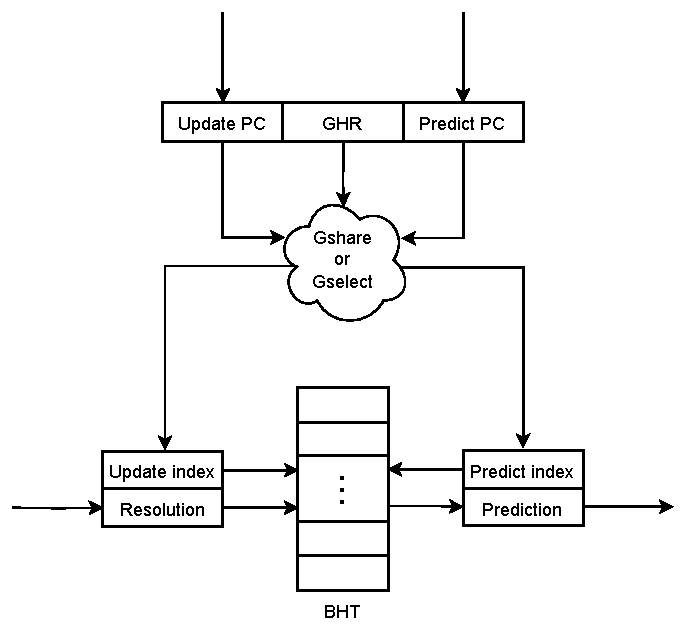
\includegraphics[width=0.8\linewidth]{media/graphics/labs_with_cva6/global_predictor.pdf}
    \caption[
        Branch Predictor Design for \enquote{Labs with CVA6}
    ]{
        Block diagram of the Global Two-Level Branch Predictor Design featured in \enquote{Labs with CVA6}.
        Participants are tasked with transforming CVA6's branch predictor into a more-sophisticated global predictor, enhancing the processor's performance by improving branch hit-rate for specifically designed benchmarks \cite{labsWithCVA6}.
    }
    \label{fig:branch_predictor}
\end{figure}


\begin{figure}[t]
    \centering
    \inputminted[frame=single]{systemverilog}{code/cache_lab/cache.svh}
    \caption{Snippet of ``Labs with CVA6'' cache lab starter code \cite{labsWithCVA6}}
    \label{fig:cache_lab}
\end{figure}


\begin{figure}[t]
    \centering

    \subfloat[
        RISC-V assembly that demonstrates out-of-order execution.
    ]{
        \begin{minipage}{0.9\textwidth}
            \large
            \inputminted{gas}{media/code/OoO.S}
        \end{minipage}
        \vspace{4pt}
    }
    \vspace{4pt}

    \subfloat[
        Screenshot of WaveForm.
        \emph{(Note: this figure omits redundant cycles to improve readability)}.
    ]{
        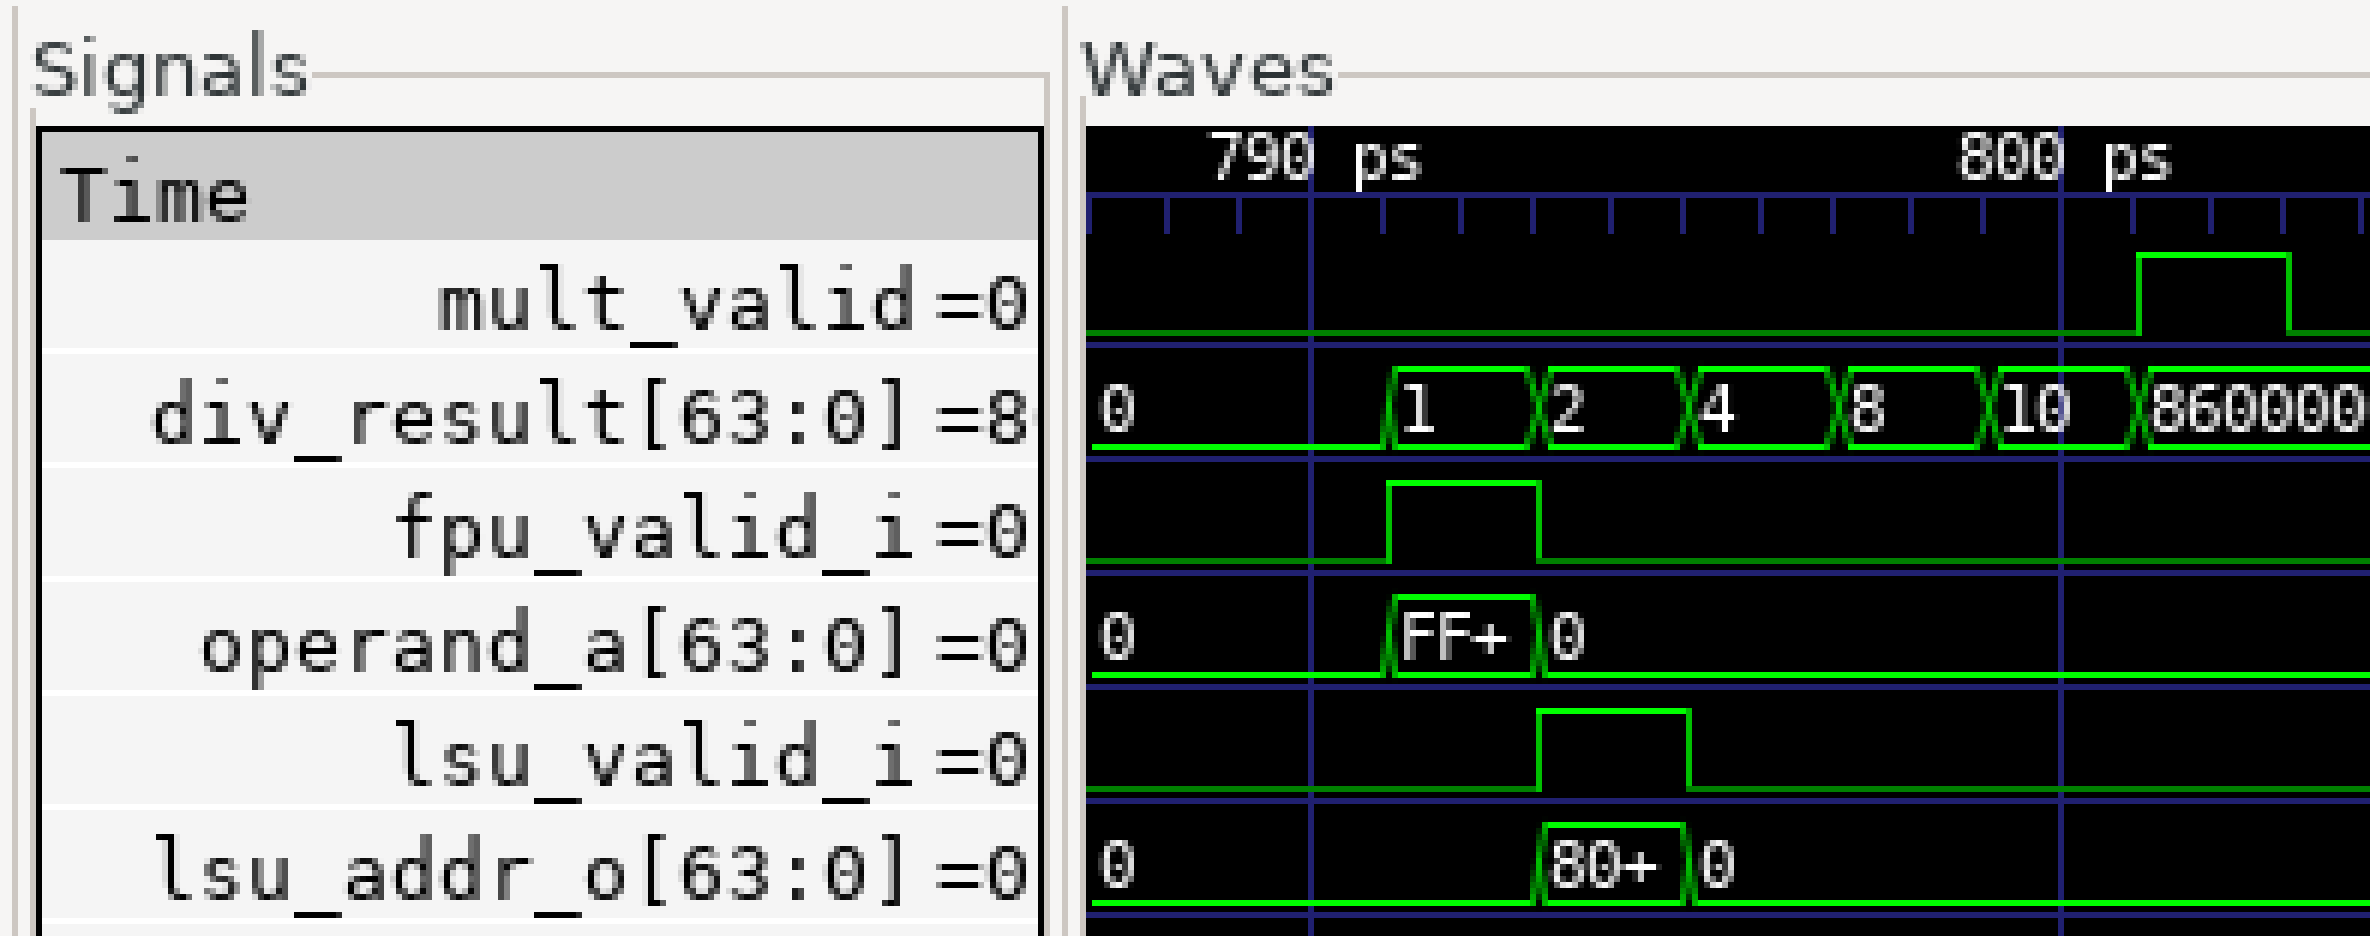
\includegraphics[width=0.9\linewidth]{media/graphics/labs_with_cva6/OoO.png}
    }
    \vspace{6pt}

    \caption[
        Out-of-Order Demonstration with CVA6
    ]{
        Out-of-Order Demonstration with CVA6: FPU and LSU finish before MULT \cite{SiffermanLatchUp}.
        In the Out-of-Order lab, participants are asked to write an assembly program to demonstrate code with and without different data-hazards.
    }
    \label{fig:OoO}

\end{figure}


\begin{figure}[t]
    \centering

    \subfloat[
        Digram provided to students to demonstrate how to move between privilege modes \cite{danielmangumRISCVPriv}.
    ]{
        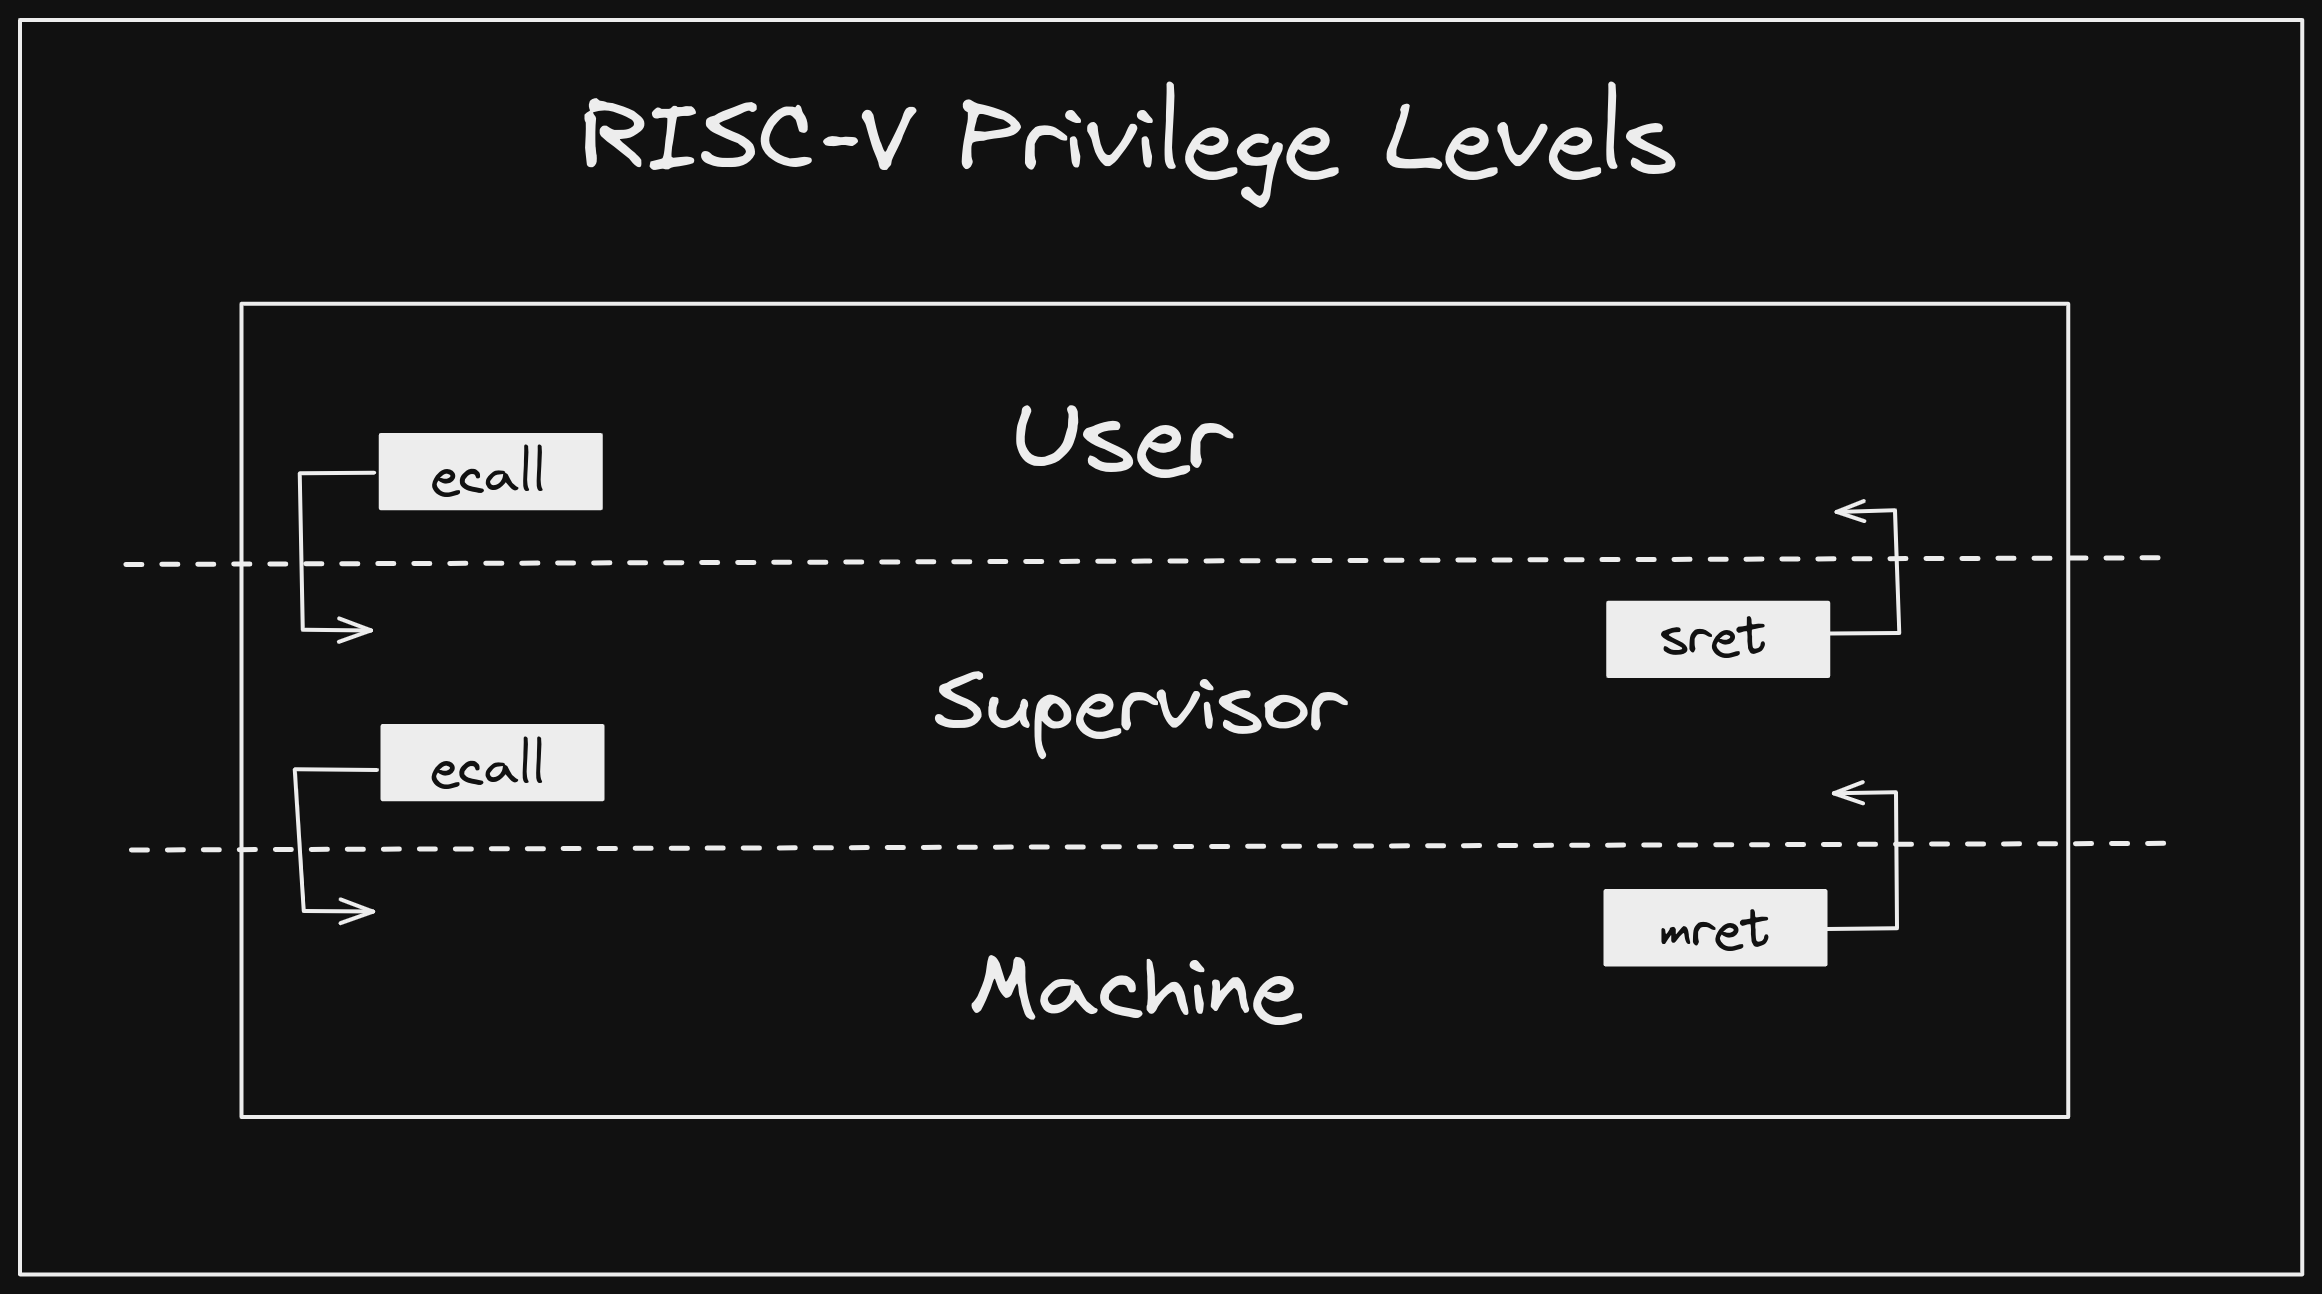
\includegraphics[width=0.8\linewidth]{media/graphics/labs_with_cva6/priv_levels.png}
    }

    \subfloat[
        Student drawing of a page table diagram
    ]{
        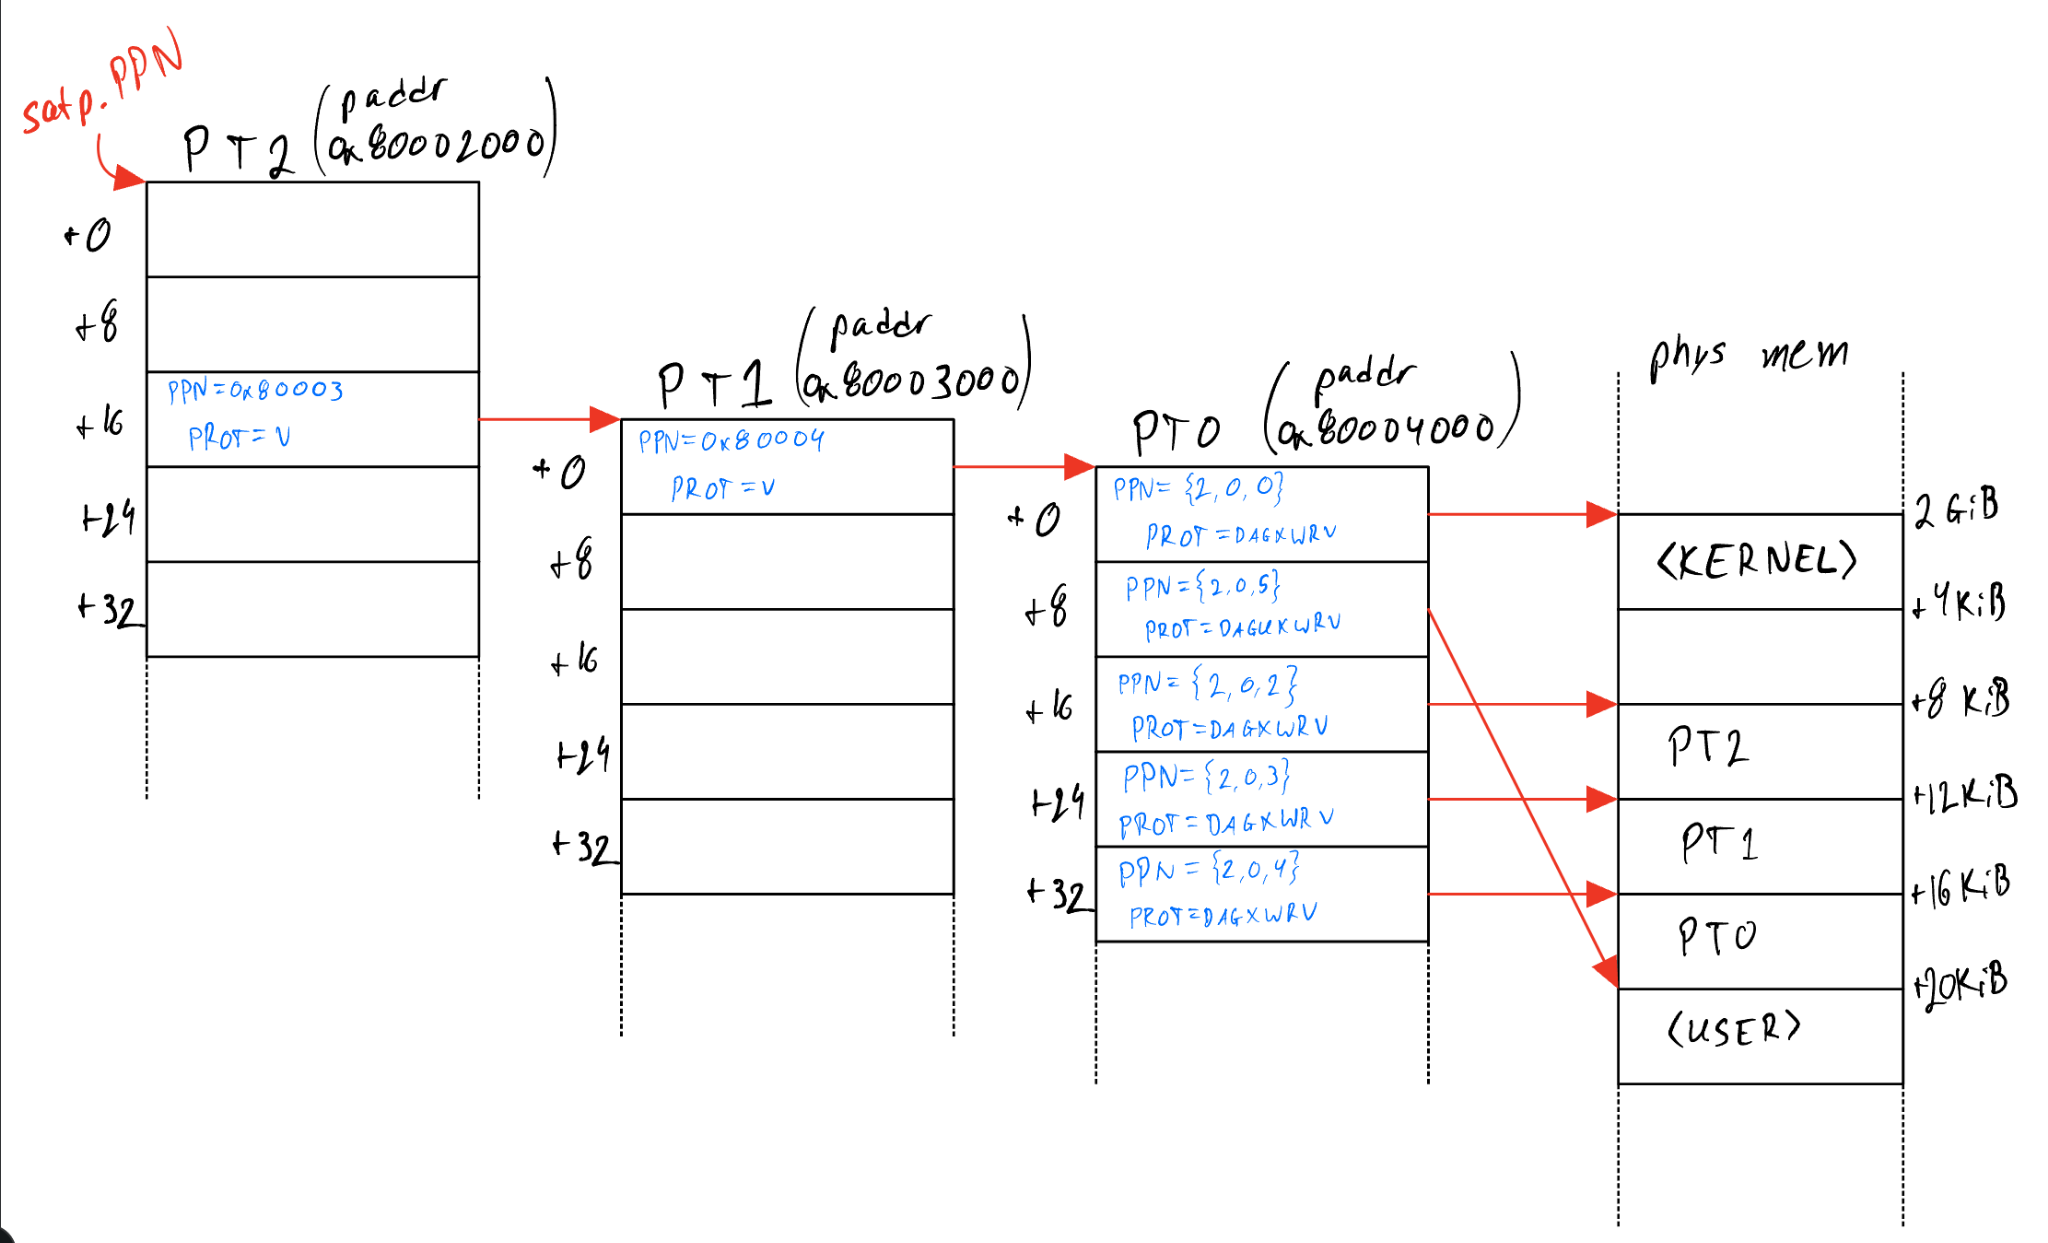
\includegraphics[width=0.8\linewidth]{media/graphics/labs_with_cva6/pt.png}
    }

    \caption[
        Virtual Memory Lab
    ]{
        Comparison of synthesis optimizations
    }
    \label{fig:virtual_memory}

\end{figure}


For instance, the Branch Prediction Lab guided students in modifying CVA6 simulations to display hit rate results and in adapting the CVA6 branch prediction unit into a global predictor (\autoref{fig:branch_predictor}). Similarly, the Caching Lab showed students how to incorporate a victim-cache module, then required creation of an assembly script to demonstrate an understanding of how the cache hierarchies and memory management would be affected (\autoref{fig:cache_lab}). Then moving away from custom RTL, in the Out-of-Order Lab, students further practiced writing assembly programs to test their comprehension of out-of-order execution by demonstrating data hazards (\autoref{fig:OoO}). Finally, the Virtual Memory Lab enabled students to configure privilege modes and set up page-table entries by modifying an assembly program that acted as a simple bootloader and OS (\autoref{fig:virtual_memory}). Each of these labs were only made possible with CVA6's open-source framework. Based on ECE 154B student responses and post-lab discussions, it was evident that the practical insights offered by these labs substantially deepen understanding of the concepts.

\FloatBarrier

\section{There is high demand for hands-on learning experiences.}

Because ``Labs with CVA6'' is available under the BSD-3-Clause license, it has attracted attention from many non-ECE 154B audiences including instructors seeking to enrich their own architecture courses, researchers aiming to familiarize themselves with the specifics of CVA6, and SystemVerilog beginners eager to learn best-practices. In addition, I gave a well-appreciated talk about ``Labs with CVA6'' at ``Latch-Up'', a conference hosted by The Free and Open Source Silicon Foundation \cite{SiffermanLatchUp}. During my presentation, I expressed the practical and unique skills that students acquire through studying the code of well-verified, open-source designs. This resonated deeply with several attendees, especially Rick O'Connor, the President and CEO at OpenHW Group, who notified me of the new RISC-V core, CV-Wally \cite{cvwally}, that is designed as a supplemental codebase for the upcoming textbook, ``RISC-V System-on-Chip Design''. The popularity that ``Labs with CVA6'' has seen, and the recent creation of CV-Wally shows that there is strong demand for curriculums that offer transparency on implementation methods of real-world designs.

\include{chapters/8_conclusion}

%=== Final ============================================


\begin{appendices}



\chapter{Open-source Contributions}
\label{appx:contributions}

This appendix identifies several open-source issues and contributions I have made.
Most of the contributions in this appendix are related to my efforts as an HDL educator.

\section{Open-source issues and contributions created by me}

\begin{itemize}
    \item [\mergedicon] \githubpull{olofk/fusesoc}{645}: Improved inheritance elaboration
    \item [\mergedicon] \githubpull{verilator/verilator}{4409}: Check for conflicting options e.g.\ \texttt{--binary} and \texttt{--lint-only}
    \item [\pullrequesticon] \githubpull{olofk/edalize}{389}: Added support for additional Verilator modes
    \item [\mergedicon] \githubpull{Rain92/FPGA-Mandelbrot}{1}: Fixed build issues
    \item [\mergedicon] \githubpull{lowRISC/style-guides}{66}: Prohibit functions from using non-local references
    \item [\mergedicon] \githubpull{steveicarus/iverilog}{980}: Argumentless functions fix
    \item [\mergedicon] \githubpull{verilator/verilator}{4172}: Added NEWERSTD warning
    \item [\mergedicon] \githubpull{openhwgroup/cva6}{1142}: Improved Acronym List in Glossary
\end{itemize}

\section{Open-source issues created by my students for my classes}

\begin{itemize}
    \item [\issueclosedicon] \githubissue{YosysHQ/oss-cad-suite-build}{28}: nextpnr-gowin support requested
\end{itemize}



\chapter{Style Guide Survey}
\label{appx:style_guides}

This appendix identifies several prominent Verilog and SystemVerilog style guides.

\section{lowRISC Verilog Coding Style Guide}

\begin{itemize}
    \item \url{https://github.com/lowRISC/style-guides} \cite{lowRISCstyleguides}
    \item Projects that use lowRISC Verilog Coding Style Guide:
    \begin{itemize}
        \item lowRISC: Ibex RISC-V Core \cite{Ibex}
        \item lowRISC: OpenTitan RISC-V Core \cite{OpenTitan}
        \item OpenHW Group: CV32E40P RISC-V Core \cite{cv32e40p}
        \item OpenHW Group: CVA6 RISC-V Core \cite{cva6}
        \item OpenHW Group: FPnew Floating-Point Unit \cite{cvfpu}
        \item PULP Platform: Ara Vector Unit \cite{Ara}
        \item PULP Platform: MemPool Many-Core System \cite{MemPool}
    \end{itemize}
\end{itemize}

\pagebreak

\section{BSG System Verilog Coding Standards}

\begin{itemize}
    \item {\fontsize{9}{12} \url{https://docs.google.com/document/d/1xA5XUzBtz_D6aSyIBQUwFk_kSUdckrfxa2uzGjMgmCU}} \cite{BSGstyleguide}
    \item Projects that use BSG System Verilog Coding Standards:
    \begin{itemize}
        \item Bespoke Silicon Group: BlackParrot RISC-V Core \cite{blackparrot}
        \item Bespoke Silicon Group: BaseJump Standard Template Library \cite{basejumpstl}
    \end{itemize}
\end{itemize}

\section{Company-Provided Style Guides}

\begin{itemize}
    \item Xilinx -- HDL Coding Techniques \cite{Xilinxstyleguide}
    \item Intel -- Recommended HDL Coding Styles \cite{Intelstyleguide}
    \item Lattice -- HDL Coding Guidelines \cite{Latticestyleguide}
    \item Freescale -- Verilog HDL Coding \cite{Freescalestyleguide}
\end{itemize}

\section{Miscellaneous Style Guides}

\begin{itemize}
    \item RSD RISC-V Core -- Coding conventions \cite{RSDstyleguide}
    \item VeriGPU -- Coding guidelines \cite{VeriGPUstyleguide}
\end{itemize}



\end{appendices}

\include{final/glossary}

\end{mainmatter}

\ssp
\bibliographystyle{JHEP3}
\bibliography{thesis}


\end{document}
